
\subsection*{\label{sub:GA_INITIALIZE}GA\_INITIALIZE}
\begin{verbatim}
\textcolor{red}{void~GA\_Initialize()}
\end{verbatim}
Allocate and initialize internal data structures in Global Arrays.

This is a collective operation. 


\subsection*{\label{sub:GA_INITIALIZE_LTD}GA\_INITIALIZE\_LTD}
\begin{verbatim}
\textcolor{red}{void~GA\_Initialize\_ltd(size\_t~limit)}



limit~amount~of~memory~in~bytes~per~process~\textcolor{green}{{[}input{]}}
\end{verbatim}
Allocate and initialize internal data structures and set limit for
memory used in global arrays. The limit is per process: it is the
amount of memory that the given processor can contribute to collective
allocation of global arrays. It does not include temporary storage
that GA might be allocating (and releasing) during execution of a
particular operation.

\emph{{*}limit }< 0 means \textquotedbl{}allow unlimited memory usage\textquotedbl{}
in which case this operation is equivalent to GA\_initialize.

This is a collective operation. 


\subsection*{\label{sub:GA_PGROUP_CREATE}GA\_PGROUP\_CREATE}
\begin{verbatim}
\textcolor{red}{int~GA\_Pgroup\_create(int~{*}list,~int~size)}



list{[}size{]}~list~of~processor~IDs~in~group~\textcolor{green}{{[}input{]}~}

size~~~~~~~number~of~processors~in~group~~\textcolor{green}{{[}input{]}}
\end{verbatim}
This command is used to create a processor group. At present, it must
be invoked by all processors in the current default processor group.
The list of processors use the indexing scheme of the default processor
group. If the default processor group is the world group, then these
indices are the usual processor indices. This function returns a process
group handle that can be used to reference this group by other functions.

This is a collective operation on the default processor group. 


\subsection*{\label{sub:GA_PGROUP_DESTROY}GA\_PGROUP\_DESTROY}
\begin{verbatim}
\textcolor{red}{int~GA\_Pgroup\_destroy(int~p\_handle)}



p\_handle~processor~group~handle~\textcolor{green}{{[}input{]}}
\end{verbatim}
This command is used to free up a processor group handle. It returns
0 if the processor group handle was not previously active.

This is a collective operation on the default processor group. 


\subsection*{\label{sub:GA_PGROUP_SET_DEFAULT}GA\_PGROUP\_SET\_DEFAULT}
\begin{verbatim}
\textcolor{red}{void~GA\_Pgroup\_set\_default(int~p\_handle)}



p\_handle~~~~~~processor~group~handle~~~~~~\textcolor{green}{{[}input{]}}
\end{verbatim}
This function can be used to reset the default processor group on
a collection of processors. All processors in the group referenced
by p\_handle must make a call to this function. Any standard global
array call that is made after resetting the default processor group
will be restricted to processors in that group. Global arrays that
are created after resetting the default processor group will only
be defined on that group and global operations such as GA\_Sync or
GA\_Igop will be restricted to processors in that group. The GA\_Pgroup\_set\_default
call can be used to rapidly convert large applications, written with
GA, into routines that run on processor groups.

The default processor group can be overridden by using GA calls that
require an explicit group handle as one of the arguments.

This is a collective operation on the group represented by the handle
p\_handle. 


\subsection*{\label{sub:NGA_CREATE}NGA\_CREATE}
\begin{verbatim}
\textcolor{red}{int~NGA\_Create(int~type,~int~ndim,~int~dims{[}{]},~char~{*}array\_name,~int~chunk{[}{]})}



array\_name~~~~~~-~a~unique~character~string~~~~~~~~~~~~~~~\textcolor{green}{{[}input{]}~}

type~~~~~~~~~~~~-~data~type~(MT\_F\_DBL,MT\_F\_INT,MT\_F\_DCPL)~\textcolor{green}{{[}input{]}~}

ndim~~~~~~~~~~~~-~number~of~array~dimensions~~~~~~~~~~~~~~\textcolor{green}{{[}input{]}}~

dims{[}ndim{]}~~~~~~-~array~of~dimensions~~~~~~~~~~~~~~~~~~~~~\textcolor{green}{{[}input{]}~}

chunk{[}ndim{]}~~~~~-~array~of~chunks,~each~element~specifies~minimum~

~~~~~~~~~~~~~~~~~~size~that~given~dimensions~should~be~chunked~

~~~~~~~~~~~~~~~~~~up~into~~~~~~~~~~~~~~~~~~~~~~~~~~~~~~~~~\textcolor{green}{{[}input{]}}
\end{verbatim}
Creates an \emph{ndim}-dimensional array using the regular distribution
model and returns integer handle representing the array.

The array can be distributed evenly or not. The control over the distribution
is accomplished by specifying \emph{chunk} (block) size for all or
some of array dimensions. For example, for a 2-dimensional array,
setting \emph{chunk{[}0{]}=dim{[}0{]}} gives distribution by vertical
strips (\emph{chunk{[}0{]}{*}dims{[}0{]}}); setting \emph{chunk{[}1{]}=dim{[}1{]}}
gives distribution by horizontal strips (\emph{chunk{[}1{]}{*}dims{[}1{]}}).
Actual chunks will be modified so that they are at least the size
of the minimum and each process has either zero or one chunk. Specifying
\emph{chunk{[}i{]} }as <1 will cause that dimension to be distributed
evenly.

As a convenience, when \emph{chunk} is specified as NULL, the entire
array is distributed evenly.

Return value: a non-zero array handle means the call was succesful.
This is a collective operation.


\subsection*{\label{sub:NGA_CREATE_CONFIG}NGA\_CREATE\_CONFIG}
\begin{verbatim}
\textcolor{red}{int~NGA\_Create\_config(int~type,~int~ndim,~int~dims{[}{]},~}

\textcolor{red}{char~{*}array\_name,~int~chunk{[}{]},~int~p\_handle)}



array\_name~~~~~~-~a~unique~character~string~~~~~~~~~~~~~~~\textcolor{green}{{[}input{]}}~

type~~~~~~~~~~~~-~data~type~(MT\_F\_DBL,MT\_F\_INT,MT\_F\_DCPL)~\textcolor{green}{{[}input{]}}~

ndim~~~~~~~~~~~~-~number~of~array~dimensions~~~~~~~~~~~~~~\textcolor{green}{{[}input{]}}~

dims{[}ndim{]}~~~~~~-~array~of~dimensions~~~~~~~~~~~~~~~~~~~~~\textcolor{green}{{[}input{]}}~

chunk{[}ndim{]}~~~~~-~array~of~chunks,~each~element~specifies~minimum~

size~that~given~dimensions~should~be~chunked~up~into~~~~~~\textcolor{green}{{[}input{]}~}

p\_handle~~~~~~~~-~processor~list~handle~~~~~~~~~~~~~~~~~~~\textcolor{green}{{[}input{]}}
\end{verbatim}
Creates an ndim-dimensional array using the regular distribution model
but with an explicitly specified processor list handle and returns
an integer handle representing the array.

This call is essentially the same as the NGA\_Create call, except
for the processor list handle \emph{p\_handle.} It can be used to
create mirrored arrays.

Return value: a non-zero array handle means the call was succesful. 

This is a collective operation. 


\subsection*{\label{sub:NGA_CREATE_GHOSTS}NGA\_CREATE\_GHOSTS}
\begin{verbatim}
\textcolor{red}{int~NGA\_Create\_ghosts(int~type,~int~ndim,~int~dims{[}{]},~int~width{[}{]},~}

\textcolor{red}{char~{*}array\_name,~int~chunk{[}{]})}



array\_name~~~-~a~unique~character~string~~~~~~~~~~~~~~~~\textcolor{green}{{[}input{]}}~

type~~~~~~~~~-~data~type~(MT\_DBL,MT\_INT,MT\_DCPL)~~~~~~~~\textcolor{green}{{[}input{]}~}

ndim~~~~~~~~~-~number~of~array~dimensions~~~~~~~~~~~~~~~\textcolor{green}{{[}input{]}}~

dims{[}ndim{]}~~~-~array~of~dimensions~~~~~~~~~~~~~~~~~~~~~~\textcolor{green}{{[}input{]}}~

width{[}ndim{]}~~-~array~of~ghost~cell~widths~~~~~~~~~~~~~~~\textcolor{green}{{[}input{]}~}

chunk{[}ndim{]}~~-~array~of~chunks,~each~element~specifies~minimum

size~that~given~dimensions~should~be~chunked~up~into~~~\textcolor{green}{{}~{[}input{]}}
\end{verbatim}
Creates an ndim-dimensional array with a layer of ghost cells around
the visible data on each processor using the regular distribution
model and returns an integer handle representing the array.

The array can be distributed evenly or not evenly. The control over
the distribution is accomplished by specifying chunk (block) size
for all or some of the array dimensions. For example, for a 2-dimensional
array, setting chunk(1)=dim(1) gives distribution by vertical strips
(chunk(1){*}dims(1)); setting chunk(2)=dim(2) gives distribution by
horizontal strips (chunk(2){*}dims(2)). Actual chunks will be modified
so that they are at least the size of the minimum and each process
has either zero or one chunk. Specifying \emph{chunk(i)} as <1 will
cause that dimension (i-th) to be distributed evenly. The width of
the ghost cell layer in each dimension is specified using the array
width(). The local data of the global array residing on each processor
will have a layer width{[}n{]} ghosts cells wide on either side of
the visible data along the dimension n.

Return value: a non-zero array handle means the call was successful.
This is a collective operation.


\subsection*{\label{sub:NGA_CREATE_GHOSTS_CONFIG}NGA\_CREATE\_GHOSTS\_CONFIG}
\begin{verbatim}
int~NGA\_Create\_ghosts\_config(int~type,~int~ndim,~int~dims{[}{]},~

int~width{[}{]},~char~{*}array\_name,~int~chunk{[}{]},~int~p\_handle)



array\_name~~-~a~unique~character~string~~~~~~~~~~~~~~~~~~{[}input{]}~

type~~~~~~~~-~data~type~(MT\_DBL,MT\_INT,MT\_DCPL)~~~~~~~~~~{[}input{]}~

ndim~~~~~~~~-~number~of~array~dimensions~~~~~~~~~~~~~~~~~{[}input{]}~

dims{[}ndim{]}~~-~array~of~dimensions~~~~~~~~~~~~~~~~~~~~~~~~{[}input{]}~

width{[}ndim{]}~-~array~of~ghost~cell~widths~~~~~~~~~~~~~~~~~{[}input{]}~

chunk{[}ndim{]}~-~array~of~chunks,~each~element~specifies~minimum~

size~that~given~dimensions~should~be~chunked~up~into~~~~~{[}input{]}~

p\_handle~~~~-~processor~list~handle
\end{verbatim}
Creates an ndim-dimensional array with a layer of ghost cells around
the visible data on each processor using the regular distribution
model and an explicitly specified processor list and returns an integer
handle representing the array.

This call is essentially the same as the NGA\_Create\_ghosts call,
except for the processor list handle \emph{p\_handle}. It can be used
to create mirrored arrays.

Return value: a non-zero array handle means the call was successful.
This is a collective operation. 


\subsection*{\label{sub:NGA_CREATE_IRREG}NGA\_CREATE\_IRREG}
\begin{verbatim}
int~NGA\_Create\_irreg(int~type,~int~ndim,~int~dims{[}{]},~char~{*}array\_name,~int~block{[}{]},~int~map{[}{]})



array\_name~-~a~unique~character~string~{[}input{]}~

type~-~MA~data~type~(MT\_F\_DBL,MT\_F\_INT,MT\_F\_DCPL)~{[}input{]}~

ndim~-~number~of~array~dimensions~{[}input{]}~

dims~-~array~of~dimension~values~{[}input{]}~

nblock{[}ndim{]}~-~no.~of~blocks~each~dimension~is~divided~into~{[}input{]}~

map{[}s{]}~-~starting~index~for~for~each~block;~the~size~

~~~~~~~~~s~is~a~sum~all~elements~of~nblock~array~{[}input{]}
\end{verbatim}
Creates an array by following the user-specified distribution and
returns integer handle representing the array.

The distribution is specified as a Cartesian product of distributions
for each dimension. The array indices start at 0. For example, the
following figure demonstrates distribution of a 2-dimensional array
8x10 on 6 (or more) processors. \emph{nblock{[}2{]}=\{3,2\}}, the
size of map array is \emph{s=5} and array map contains the following
elements \emph{map=\{0,2,6, 0, 5\}}. The distribution is nonuniform
because, P1 and P4 get 20 elements each and processors P0,P2,P3, and
P5 only 10 elements each. 

\begin{tabular}{|c|c|c|}
\cline{1-2} 
5 & 5 & \multicolumn{1}{c}{}\tabularnewline
\hline 
P0 & P3 & 2\tabularnewline
\hline 
P1 & P4 & 4\tabularnewline
\hline 
P2 & P5 & 2\tabularnewline
\hline
\end{tabular}

Return value: a non-zero array handle means the call was succesful.
This is a collective operation.


\subsection*{\label{sub:NGA_CREATE_IRREG_CONFIG}NGA\_CREATE\_IRREG\_CONFIG}
\begin{verbatim}
int~NGA\_Create\_irreg\_config(int~type,~int~ndim,~int~dims{[}{]},

char~{*}array\_name,~int~block{[}{]},~int~map{[}{]},~int~p\_handle)



array\_name~~~-~a~unique~character~string~~~~~~~~~~~~~~~~~~~~{[}input{]}~

type~~~~~~~~~-~MA~data~type~(MT\_F\_DBL,MT\_F\_INT,MT\_F\_DCPL)~~~{[}input{]}~

ndim~~~~~~~~~-~number~of~array~dimensions~~~~~~~~~~~~~~~~~~~{[}input{]}~

dims~~~~~~~~~-~array~of~dimension~values~~~~~~~~~~~~~~~~~~~~{[}input{]}~

nblock{[}ndim{]}~-~no.~of~blocks~each~dimension~is~divided~into~{[}input{]}~

map{[}s{]}~~~~~~~-~starting~index~for~for~each~block;~the~size~

~~~~~~~~~~~~~~~s~is~a~sum~all~elements~of~nblock~array~~~~~~{[}input{]}~

p\_handle~~~~~-~processor~list~handle
\end{verbatim}
Creates an array by following the user-specified distribution and
an explicitly specified processor list handle and returns an integer
handle representing the array.

This call is essentially the same as the NGA\_Create\_irreg call,
except for the processor list handle p\_handle. It can be used to
create mirrored arrays.

Return value: a non-zero array handle means the call was succesful.
This is a collective operation. 


\subsection*{\label{sub:NGA_CREATE_GHOST_IRREG}NGA\_CREATE\_GHOST\_IRREG}
\begin{verbatim}
int~NGA\_Create\_ghost\_irreg(int~type,~int~ndim,~int~dims{[}{]},~

width{[}{]},~char~{*}array\_name,~map{[}{]},~nblock{[}{]})



array\_name~~~-~a~unique~character~string~~~~~~~~~~~~~~~~~~~{[}input{]}

type~~~~~~~~~-~data~type~(MT\_DBL,MT\_INT,MT\_DCPL)~~~~~~~~~~~{[}input{]}~

ndim~~~~~~~~~-~number~of~array~dimensions~~~~~~~~~~~~~~~~~~{[}input{]}~

dims{[}ndim{]}~~~-~array~of~dimensions~~~~~~~~~~~~~~~~~~~~~~~~~{[}input{]}~

width{[}ndim{]}~~-~array~of~ghost~cell~widths~~~~~~~~~~~~~~~~~~{[}input{]}~

nblock{[}ndim{]}~-~no.~of~blocks~each~dimension~is~divided~into{[}input{]}~

map{[}s{]}~~~~~~~-~starting~index~for~for~each~block;~the~size~s~

~~~~~~~~~~~~~~~is~a~sum~of~all~elements~of~nblock~array~~~~{[}input{]}
\end{verbatim}
Creates an array with ghost cells by following the user-specified
distribution and returns integer handle representing the array.

The distribution is specified as a Cartesian product of distributions
for each dimension. For example, the following figure demonstrates
distribution of a 2-dimensional array 8x10 on 6 (or more) processors.
nblock(2)=\{3,2\}, the size of map array is s=5 and array map contains
the following elements map=\{1,3,7, 1, 6\}. The distribution is nonuniform
because, P1 and P4 get 20 elements each and processors P0,P2,P3, and
P5 only 10 elements each. 

\begin{tabular}{|c|c|c|}
\cline{1-2} 
5 & 5 & \multicolumn{1}{c}{}\tabularnewline
\hline 
P0 & P3 & 2\tabularnewline
\hline 
P1 & P4 & 4\tabularnewline
\hline 
P2 & P5 & 2\tabularnewline
\hline
\end{tabular} 

The array width{[}{]} is used to control the width of the ghost cell
boundary around the visible data on each processor. The local data
of the global array residing on each processor will have a layer width{[}n{]}
ghosts cells wide on either side of the visible data along the dimension
n.

Return value: a non-zero array handle means the call was succesful.
This is a collective operation.


\subsection*{\label{sub:NGA_CREATE_GHOSTS_IRREG_CONFIG}NGA\_CREATE\_GHOSTS\_IRREG\_CONFIG}
\begin{verbatim}
int~NGA\_Create\_ghost\_irreg\_config(int~type,~int~ndim,~int~dims{[}{]},

width{[}{]},~char~{*}array\_name,~map{[}{]},~nblock{[}{]},~int~p\_handle)



array\_name~~~-~a~unique~character~string~~~~~~~~~~~~~~~~~~~{[}input{]}~

type~~~~~~~~~-~data~type~(MT\_DBL,MT\_INT,MT\_DCPL)~~~~~~~~~~~{[}input{]}~

ndim~~~~~~~~~-~number~of~array~dimensions~~~~~~~~~~~~~~~~~~{[}input{]}~

dims{[}ndim{]}~~~-~array~of~dimensions~~~~~~~~~~~~~~~~~~~~~~~~~{[}input{]}

width{[}ndim{]}~~-~array~of~ghost~cell~widths~~~~~~~~~~~~~~~~~~{[}input{]}~

nblock{[}ndim{]}~-~no.~of~blocks~each~dimension~is~divided~into{[}input{]}~

map{[}s{]}~~~~~~~-~starting~index~for~for~each~block;~the~size~s~

~~~~~~~~~~~~~~~is~a~sum~of~all~elements~of~nblock~array~~~~{[}input{]}~

p\_handle~~~~~-~processor~list~handle~~~~~~~~~~~~~~~~~~~~~~~{[}input{]}
\end{verbatim}
Creates an array with ghost cells by following the user-specified
distribution and returns integer handle representing the array.

This call is essentially the same as the NGA\_Create\_ghosts\_irreg
call, except for the processor list handle \emph{p\_handle}. It can
be used to create mirrored arrays.

Return value: a non-zero array handle means the call was succesful.

This is a collective operation. 


\subsection*{\label{sub:GA_CREATE_HANDLE}GA\_CREATE\_HANDLE}
\begin{verbatim}
int~GA\_Create\_handle()6
\end{verbatim}
This function returns a global array handle that can then be used
to create a new global array. This is part of a new API for creating
global arrays that is designed to replace the old interface built
around the NGA\_Create\_xxx calls. The sequence of operations is to
begin with a call to GA\_Greate\_handle to get a new array handle.
The attributes of the array, such as dimension, size, type, etc. can
then be set using successive calls to the GA\_Set\_xxx subroutines.
When all array attributes have been set, the GA\_Allocate subroutine
is called and the global array is actually created and memory for
it is allocated.

This is a collective operation. 


\subsection*{\label{sub:GA_SET_ARRAY_NAME}GA\_SET\_ARRAY\_NAME}
\begin{verbatim}
void~GA\_Set\_array\_name(int~g\_a,~char~{*}name)



g\_a~{[}input{]}~name~-~array~name~{[}input{]}
\end{verbatim}
This function can be used to assign a unique character string name
to a global array handle that was obtained using the GA\_Create\_handle
function.

This is a collective operation. 


\subsection*{\label{sub:GA_SET_DATA}GA\_SET\_DATA}
\begin{verbatim}
void~GA\_Set\_data(int~g\_a,~int~ndim,~int~dims{[}{]},~int~type)



g\_a~{[}input{]}~ndim~-~dimension~of~global~array~~{[}input{]}~

dims{[}{]}~~~~~~~~~~~-~dimensions~of~global~array~{[}input{]}~

type~~~~~~~~~~~~~-~data~type~of~global~array~~{[}input{]}
\end{verbatim}
This function can be used to set the array dimension, the coordinate
dimensions, and the data type assigned to a global array handle obtained
using the GA\_Create\_handle function.

This is a collective operation. 


\subsection*{\label{sub:GA_SET_IRREG_DISTR}GA\_SET\_IRREG\_DISTR}
\begin{verbatim}
void~GA\_Set\_irreg\_distr(int~g\_a,~int~mapc{[}{]},~int~nblock{[}{]})



g\_a~~~~~~~~~~~~~~~~~~~~~~~~~~~~~~~~~~~~~~~~~~~~{[}input{]}~

mapc{[}s{]}~~~~~~~-~starting~index~for~each~block;~

~~~~~~~~~~~~~~~~the~size~s~is~the~sum~of~all~

~~~~~~~~~~~~~~~~elements~of~the~array~nblock~~~{[}input{]}~

nblock{[}ndim{]}~-~number~of~blocks~that~each~dimension~

~~~~~~~~~~~~~~~is~divided~into~~~~~~~~~~~~~~~~~{[}input{]}
\end{verbatim}
This function can be used to partition the array data among the individual
processors for a global array handle obtained using the GA\_Create\_handle
function.

The distribution is specified as a Cartesian product of distributions
for each dimension. For example, the following figure demonstrates
distribution of a 2-dimensional array 8x10 on 6 (or more) processors.
nblock(2)=\{3,2\}, the size of mapc array is s=5 and array mapc contains
the following elements mapc=\{1,3,7, 1, 6\}. The distribution is nonuniform
because, P1 and P4 get 20 elements each and processors P0,P2,P3, and
P5 only 10 elements each. 

\begin{tabular}{|c|c|c|}
\cline{1-2} 
5 & 5 & \multicolumn{1}{c}{}\tabularnewline
\hline 
P0 & P3 & 2\tabularnewline
\hline 
P1 & P4 & 4\tabularnewline
\hline 
P2 & P5 & 2\tabularnewline
\hline
\end{tabular} 

The array width() is used to control the width of the ghost cell boundary
around the visible data on each processor. The local data of the global
array residing on each processor will have a layer width(n) ghosts
cells wide on either side of the visible data along the dimension
n.

This is a collective operation. 


\subsection*{\label{sub:GA_SET_PGROUP}GA\_SET\_PGROUP}
\begin{verbatim}
void~GA\_Set\_pgroup(int~g\_a,~int~p\_handle)



g\_a~~~~~~~~~~~~~~~~~~~~~~~~~~~~~{[}input{]}~

p\_handle~processor~group~handle~{[}input{]}
\end{verbatim}
This function can be used to set the processor configuration assigned
to a global array handle that was obtained using the GA\_Create\_handlefunction.
It can be used to create mirrored arrays by using the mirrored array
processor configuration in this function call. It can also be used
to create an array on a processor group by using a processor group
handle in this call.

This is a collective operation. 


\subsection*{\label{sub:GA_SET_GHOSTS}GA\_SET\_GHOSTS}
\begin{verbatim}
void~GA\_Set\_ghosts(int~g\_a,~int~width{[}{]})



g\_a~{[}input{]}~width{[}ndim{]}~-~array~of~ghost~cell~widths~{[}input{]}
\end{verbatim}
This function can be used to set the ghost cell widths for a global
array handle that was obtained using the GA\_Create\_handle function.
The ghosts cells widths indicate how many ghost cells are used to
pad the locally held array data along each dimension. The padding
can be set independently for each coordinate dimension.

This is a collective operation. 


\subsection*{\label{sub:GA_SET_CHUNK}GA\_SET\_CHUNK}
\begin{verbatim}
void~GA\_Set\_chunk(int~g\_a,~int~chunk{[}{]})



g\_a~~~~~~~~~~~~~~~~~~~~~~~~~~~~~{[}input{]}~

chunk{[}{]}~-~array~of~chunk~widths~{[}input{]}
\end{verbatim}
This function is used to set the chunk array for a global array handle
that was obtained using the GA\_Create\_handle function. The chunk
array is used to determine the minimum number of array elements assigned
to each processor along each coordinate direction.

This is a collective operation. 


\subsection*{\label{sub:GA_SET_BLOCK_CYCLIC}GA\_SET\_BLOCK\_CYCLIC}
\begin{verbatim}
void~GA\_Set\_block\_cyclic(int~g\_a,~int~dims{[}{]})



g\_a~~~~-~global~array~handle~~~~~~~~~~{[}input{]}~

dims{[}{]}~-~array~of~block~dimensions~~~~{[}input{]}
\end{verbatim}
This subroutine is used to create a global array with a simple block-cyclic
data distribution. The array is broken up into blocks of size dims
and each block is numbered sequentially using a column major indexing
scheme. The blocks are then assigned in a simple round-robin fashion
to processors. This is illustrated in the figure below for an array
containing 25 blocks distributed on 4 processors. Blocks at the edge
of the array may be smaller than the block size specified in dims.
In the example below, blocks 4,9,14,19,20,21,22,23, and 24 might be
smaller thatn the remaining blocks. Most global array operations are
insensitive to whether or not a block-cyclic data distribution is
used, although performance may be slower in some cases if the global
array is using a block-cyclic data distribution. Individual data blocks
can be accessesed using the block-cyclic access functions.

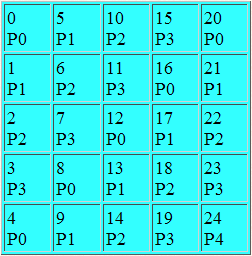
\includegraphics{Set_Block_Cyclic}

This is a collective operation. 


\subsection*{\label{sub:GA_SET_BLOCK_CYCLIC_PROC_GRID}GA\_SET\_BLOCK\_CYCLIC\_PROC\_GRID}
\begin{verbatim}
void~GA\_Set\_block\_cyclic(int~g\_a,~int~dims{[}{]},~int~proc\_grid{[}{]})



g\_a~~~~~~~~~-~global~array~handle~~~~~~~{[}input{]}~

dims{[}{]}~~~~~~-~array~of~block~dimensions~{[}input{]}~

proc\_grid{[}{]}~-~processor~grid~dimensions~{[}input{]}
\end{verbatim}
This subroutine is used to create a global array with a SCALAPACK-type
block cyclic data distribution. The user specifies the dimensions
of the processor grid in the array proc\_grid. The product of the
processor grid dimensions must equal the number of total number of
processors and the number of dimensions in the processor grid must
be the same as the number of dimensions in the global array. The data
blocks are mapped onto the processor grid in a cyclic manner along
each of the processor grid axes. This is illustrated below for an
array consisting of 25 data blocks disributed on 6 processors. The
6 processors are configured in a 3 by 2 processor grid. Blocks at
the edge of the array may be smaller than the block size specified
in dims. Most global array operations are insensitive to whether or
not a block-cyclic data distribution is used, although performance
may be slower in some cases if the global array is using a block-cyclic
data distribution. Individual data blocks can be accessesed using
the block-cyclic access functions.

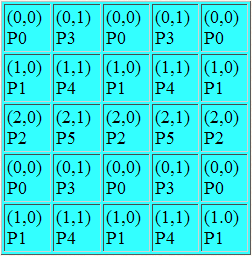
\includegraphics{Set_Block_Cyclic_Proc_Grid}

This is a collective operation.


\subsection*{\label{sub:GA_ALLOCATE}GA\_ALLOCATE}
\begin{verbatim}
int~GA\_Allocate(int~g\_a)



g\_a~~~~~~~~~~~~~~{[}input{]}
\end{verbatim}
This function allocates the memory for the global array handle originally
obtained using the GA\_Create\_handle function. At a minimum, the
GA\_Set\_data function must be called before the memory is allocated.
Other GA\_Set\_xxx functions can also be called before invoking this
function.

This is a collective operation. 


\subsection*{\label{sub:GA_UPDATE_GHOSTS}GA\_UPDATE\_GHOSTS}
\begin{verbatim}
void~GA\_Update\_ghosts(int~g\_a)
\end{verbatim}
This call updates the ghost cell regions on each processor with the
corresponding neighbor data from other processors. The operation assumes
that all data is wrapped around using periodic boundary data so that
ghost cell data that goes beyound an array boundary is wrapped around
to the other end of the array. The GA\_Update\_ghosts call contains
two GA\_Sync calls before and after the actual update operation. For
some applications these calls may be unecessary, if so they can be
removed using the GA\_Mask\_sync subroutine. This is a collective
operation. 


\subsection*{\label{sub:NGA_UPDATE_GHOST_DIR}NGA\_UPDATE\_GHOST\_DIR}
\begin{verbatim}
int~NGA\_Update\_ghost\_dir(int~g\_a,~int~dimension,~int~idir,~int~cflag)



g\_a~~~~~~~~~~~~~~~~~~~~~~~~~~~~~~~~~~~~~~~~~~~~~~~~~{[}input{]}~

dimension~-~array~dimension~that~is~to~be~updated~~~{[}input{]}~

idir~~~~~~-~direction~of~update~(+/-~1)~~~~~~~~~~~~~{[}input{]}~

cflag~~~~~-~flag~(0/1)~to~include~corners~in~update~{[}input{]}
\end{verbatim}
This function can be used to update the ghost cells along individual
directions. It is designed for algorithms that can overlap updates
with computation. The variable dimension indicates which coordinate
direction is to be updated (e.g. dimension = 1 would correspond to
the y axis in a two or three dimensional system), the variable idir
can take the values +/-1 and indicates whether the side that is to
be updated lies in the positive or negative direction, and cflag indicates
whether or not the corners on the side being updated are to be included
in the update. The following calls would be equivalent to a call to
GA\_Update\_ghosts for a 2-dimensional system: 
\begin{verbatim}
status~=~NGA\_Update\_ghost\_dir(g\_a,0,-1,1);~

status~=~NGA\_Update\_ghost\_dir(g\_a,0,1,1);~

status~=~NGA\_Update\_ghost\_dir(g\_a,1,-1,0);~

status~=~NGA\_Update\_ghost\_dir(g\_a,1,1,0);
\end{verbatim}
The variable cflag is set equal to 1 (or non-zero) in the first two
calls so that the corner ghost cells are update, it is set equal to
0 in the second two calls to avoid redundant updates of the corners.
Note that updating the ghosts cells using several independent calls
to the nga\_update\_ghost\_dir functions is generally not as efficient
as using GA\_Update\_ghosts unless the individual calls can be effectively
overlapped with computation.

This is a collective operation. 


\subsection*{\label{sub:GA_HAS_GHOSTS}GA\_HAS\_GHOSTS}
\begin{verbatim}
int~GA\_Has\_ghosts(int~g\_a)
\end{verbatim}
This function returns 1 if the global array has some dimensions for
which the ghost cell width is greater than zero, it returns 0 otherwise.
This is a collective operation. 


\subsection*{\label{sub:NGA_ACCESS_GHOSTS}NGA\_ACCESS\_GHOSTS}
\begin{verbatim}
void~NGA\_Access\_ghosts(int~g\_a,~int~dims{[}{]},~void~{*}ptr,~int~ld{[}{]})



g\_a~~~~~~~~~~~~~~~~~~~~~~~~~~~~~~~~~~~~~~~~~~~~~~~~~~~~~~~~~~~~~~~{[}input{]}~

dims{[}ndim{]}~-~array~of~dimensions~of~local~patch,~including~

~~~~~~~~~~~~~ghost~cells~~~~~~~~~~~~~~~~~~~~~~~~~~~~~~~~~~~~~~~~~~{[}output{]}~

ptr~~~~~~~~-~returns~an~index~corresponding~to~the~origin~

~~~~~~~~~~~~~the~global~array~patch~held~locally~on~the~processor~{[}output{]}~

ld{[}ndim-1{]}~-~physical~dimenstions~of~the~local~array~patch,~

~~~~~~~~~~~~~including~ghost~cells~~~~~~~~~~~~~~~~~~~~~~~~~~~~~~~~{[}output{]}
\end{verbatim}
Provides access to the local patch of the global array. Returns leading
dimension ld and and pointer for the data. This routine will provide
access to the ghost cell data residing on each processor. Calls to
NGA\_Access\_ghosts should normally follow a call to NGA\_Distribution
that returns coordinates of the visible data patch associated with
a processor. You need to make sure that the coordinates of the patch
are valid (test values returned from NGA\_Distribution).

You can only access local data. This is a local operation. 


\subsection*{\label{sub:NGA_ACCESS_GHOST_ELEMENT}NGA\_ACCESS\_GHOST\_ELEMENT}
\begin{verbatim}
void~NGA\_Access\_ghost\_element(int~g\_a,~void~{*}ptr,~int~

subscript{[}{]},~int~ld{[}{]})



g\_a~~~~~~~~~~~~~~~~~~~~~~~~~~~~~~~~~~~~~~~~~~~~~~~~~~~~~~~~~{[}input{]}~

index~~~~~~~~~~~~~~~~~~~~~~~~~~~~~~~~-~index~pointing~to~location~

~~~~~~~~~~~~~~~~~~~~~~~~~~~~~~~~~~~~~~~of~element~indexed~by~

subscript{[}{]}~{[}output{]}~subscript{[}ndim{]}~-~array~of~integers~that~index~

~~~~~~~~~~~~~~~~~~~~~~~~~~~~~~~~~~~~~~~desired~element~~~~~~{[}input{]}~

ld{[}ndim-1{]}~-~array~of~strides~for~local~data~patch.~These~include~

~~~~~~~~~~~~~~~~~~~~~~~~~~~~~~~~~~~~~~~ghost~cell~widths.~~~{[}output{]}
\end{verbatim}
This function can be used to return a pointer to any data element
in the locally held portion of the global array and can be used to
directly access ghost cell data. The array subscript refers to the
local index of the element relative to the origin of the local patch
(which is assumed to be indexed by (0,0,...)). This is a local operation. 


\subsection*{\label{sub:GA_TOTAL_BLOCKS}GA\_TOTAL\_BLOCKS}
\begin{verbatim}
int~GA\_Total\_blocks(int~g\_a)



g\_a~~~~~~~~~~~~~~~~~~{[}input{]}
\end{verbatim}
This function returns the total number of blocks contained in a global
array with a block-cyclic data distribution. This is a local operation. 


\subsection*{\label{sub:GA_GET_BLOCK_INFO}GA\_GET\_BLOCK\_INFO}
\begin{verbatim}
void~GA\_Get\_block\_info(int~g\_a,~int~num\_blocks{[}{]},~int~block\_dims{[}{]})



g\_a~~~~~~~~~~~~~~~~~~~~~~~~~~~~~~~~~~~~~~~~~~~~~~~~~{[}input{]}~

num\_blocks{[}ndim{]}~-~number~of~blocks~along~each~axis~{[}output{]}~

block\_dims{[}ndim{]}~-~dimensions~of~block~~~~~~~~~~~~~~{[}output{]}
\end{verbatim}
This subroutine returns information about the block-cyclic distribution
associated with global array g\_a. The number of blocks along each
of the array axes are returned in the array num\_blocks and the dimensions
of the individual blocks, specified in the GA\_Set\_block\_cyclic
or GA\_Set\_block\_cyclic\_proc\_grid subroutines, are returned in
block\_dims. This is a local function. 


\subsection*{\label{sub:GA_DUPLICATE}GA\_DUPLICATE}
\begin{verbatim}
int~GA\_Duplicate(int~g\_a,~char{*}~array\_name)



array\_name~-~a~character~string~~~~~~~~~~~~~~~~~{[}input{]}~

g\_a~~~~~~~~-~integer~handle~for~reference~array~{[}input{]}
\end{verbatim}
Creates a new array by applying all the properties of another existing
array. It returns array handle.

Return value: a non-zero array handle means the call was succesful.
This is a collective operation. GA\_DESTROY

void GA\_Destroy(int g\_a)

g\_a - array handle {[}input{]}

Deallocates the array and frees any associated resources.

This is a collective operation. 


\subsection*{\label{sub:GA_TERMINATE}GA\_TERMINATE}
\begin{verbatim}
void~GA\_Terminate()
\end{verbatim}
Delete all active arrays and destroy internal data structures.

This is a collective operation. 


\subsection*{\label{sub:GA_SYNC}GA\_SYNC}
\begin{verbatim}
void~GA\_Sync()
\end{verbatim}
Synchronize processes (a barrier) and ensure that all GA operations
completed.

This is a collective operation.


\subsection*{GA\_MASK\_SYNC}
\begin{verbatim}
void~GA\_Mask\_sync(int~first,int~last)



first~-~mask~(0/1)~for~prior~internal~synchronization~{[}input{]}~

last~~-~mask~(0/1)~for~post~internal~synchronization~~{[}input{]}
\end{verbatim}
This subroutine can be used to remove synchronization calls from around
collective operations. Setting the parameter first = .false. removes
the synchronization prior to the collective operation, setting last
= .false. removes the synchronization call after the collective operation.
This call is applicable to all collective operations. It most be invoked
before each collective operation. This is a collective operation. 


\subsection*{\label{sub:GA_ZERO}GA\_ZERO}
\begin{verbatim}
void~GA\_Zero(int~g\_a)



g\_a~-~array~handle~{[}input{]}
\end{verbatim}
Sets value of all elements in the array to zero.

This is a collective operation. 


\subsection*{\label{sub:GA_FILL}GA\_FILL}
\begin{verbatim}
void~GA\_Fill(int~g\_a,~void~{*}value)



g\_a~-~array~handle~~~~~~~~~~~~~~~~~~~~~~~~~~~~~~~~~~~~~~~~~~{[}input{]}~

value~-~pointer~to~the~value~of~appropriate~type~

~~~~~~~~(double/DoubleComplex/long)~that~matches~array~type~{[}input{]}
\end{verbatim}
Assign a single value to all elements in the array.

This is a collective operation. 


\subsection*{\label{sub:GA_DOT}GA\_DOT}
\begin{verbatim}
\textcolor{red}{int~GA\_Idot(int~g\_a,~int~g\_b)~}

\textcolor{red}{long~GA\_Ldot(int~g\_a,~int~g\_b)~}

\textcolor{red}{float~GA\_Fdot(int~g\_a,~int~g\_b)~}

\textcolor{red}{double~GA\_Ddot(int~g\_a,~int~g\_b)~}

\textcolor{red}{DoubleComplex~GA\_Zdot(int~g\_a,~int~g\_b)}



g\_a,~g\_b~-~array~handles~{[}input{]}
\end{verbatim}
Computes the element-wise dot product of the two arrays which must
be of the same types and same number of elements.

return value = SUM\_ij a(i,j){*}b(i,j)

This is a collective operation. 


\subsection*{\label{sub:GA_SCALE}GA\_SCALE}
\begin{verbatim}
void~GA\_Scale(int~g\_a,~void~{*}value)



g\_a~-~array~handle~~~~~~~~~~~~~~~~~~~~~~~~~~~~~~~~~~~~~~~~~~{[}input{]}~

value~-~pointer~to~the~value~of~appropriate~type~

~~~~~~~~(double/DoubleComplex/long)~that~matches~array~type~{[}input{]}
\end{verbatim}
Scales an array by the constant s. Note that the library is unable
to detect errors when the pointed value is of different type than
the array.

This is a collective operation. 


\subsection*{\label{sub:GA_ADD}GA\_ADD}
\begin{verbatim}
void~GA\_Add(void~{*}alpha,~int~g\_a,~void{*}~beta,~int~g\_b,~int~g\_c)



g\_a,~g\_b,~g\_c~~~~~~~~~~~~~-~array~handles~~~~~~~~~~~~{[}input{]}~

double/complex/int~{*}alpha~-~scale~factor~~~~~~~~~~~~~{[}input{]}

double/complex/int~{*}beta~~-~scale~factor~~~~~~~~~~~~~{[}input{]}
\end{verbatim}
The arrays (which must be the same shape and identically aligned)
are added together element-wise

\emph{c = alpha {*} a + beta {*} b.}

The result \emph{(c)} may replace one of the input arrays \emph{(a/b)}.

This is a collective operation. 


\subsection*{\label{sub:GA_COPY}GA\_COPY}
\begin{verbatim}
void~GA\_Copy(int~g\_a,~int~g\_b)



g\_a,~g\_b~-~array~handles~~~~~~~~~{[}input{]}
\end{verbatim}
Copies elements in array represented by g\_a into the array represented
by g\_b. The arrays must be the same type, shape, and identically
aligned.

This is a collective operation.


\subsection*{\label{sub:GA_SET_MEMORY_LIMIT}GA\_SET\_MEMORY\_LIMIT}
\begin{verbatim}
void~GA\_Set\_memory\_limit(size\_t~limit)



limit~-~the~amount~of~memory~in~bytes~per~process~{[}input{]}
\end{verbatim}
Sets the amount of memory to be used (in bytes) per process

This is a local operation.


\subsection*{\label{sub:GA_GET}GA\_GET}
\begin{verbatim}
void~NGA\_Get(int~g\_a,~int~lo{[}{]},~int~hi{[}{]},~void{*}~buf,~int~ld{[}{]})



g\_a~~~~~~~~-~global~array~handle~~~~~~~~~~~~~~~~~~~~~~~~~~~~~~~~{[}input{]}~

ndim~~~~~~~-~number~of~dimensions~of~the~global~array~

lo{[}ndim{]}~~~-~array~of~starting~indices~for~global~array~section~{[}input{]}

hi{[}ndim{]}~~~-~array~of~ending~indices~for~global~array~section~~~{[}input{]}

buf~-~pointer~to~the~local~buffer~array~where~the~data~goes~~~~~{[}output{]}

ld{[}ndim-1{]}~-~array~specifying~leading~dimensions/strides/extents~

~~~~~~~~~~~~~for~buffer~array~~~~~~~~~~~~~~~~~~~~~~~~~~~~~~~~~~~{[}input{]}
\end{verbatim}
Copies data from global array section to the local array buffer. The
local array is assumed to be have the same number of dimensions as
the global array. Any detected inconsitencies/errors in the input
arguments are fatal.

\emph{Example:} For ga\_get operation transfering data from the {[}10:14,0:4{]}
section of 2-dimensional 15x10 global array into local buffer 5x10
array we have: \emph{lo=\{10,0\}, hi=\{14,4\}, ld=\{10\} }

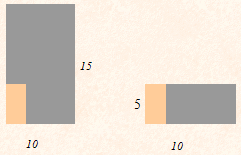
\includegraphics{GA_Get}

This is a one-sided operation.


\subsection*{\label{sub:GA_PERIODIC_GET}GA\_PERIODIC\_GET}
\begin{verbatim}
void~NGA\_Periodic\_get(int~g\_a,~int~lo{[}{]},~int~hi{[}{]},~void{*}~buf,~int~ld{[}{]})



g\_a~-~~~~~~~~global~array~handle~~~~~~~~~~~~~~~~~~~~~~~~~~~~~~~~{[}input{]}~

ndim~-~~~~~~~number~of~dimensions~of~the~global~array~

lo{[}ndim{]}~-~~~array~of~starting~indices~for~global~array~section~{[}input{]}

hi{[}ndim{]}~-~~~array~of~ending~indices~for~global~array~section~~~{[}input{]}

buf~-~pointer~to~the~local~buffer~array~where~the~data~goes~~~~~{[}output{]}

ld{[}ndim-1{]}~-~array~specifying~leading~dimensions/strides/extents~

~~~~~~~~~~~~~for~buffer~array~~~~~~~~~~~~~~~~~~~~~~~~~~~~~~~~~~~{[}input{]}
\end{verbatim}
Same as nga\_get except the indices can extend beyond the array boundary/dimensions
in which case the library wraps them around. This is a one-sided operation. 


\subsection*{\label{sub:GA_STRIDED_GET}GA\_STRIDED\_GET}
\begin{verbatim}
void~NGA\_Strided\_get(int~g\_a,~int~lo{[}{]},~int~hi{[}{]},~int~skip{[}{]},~

void{*}~buf,~int~ld{[}{]})



g\_a~~~~~~~~-~global~array~handle~~~~~~~~~~~~~~~~~~~~~~~~~~~~~~~~{[}input{]}~

ndim~~~~~~~-~number~of~dimensions~of~the~global~array~

lo{[}ndim{]}~~~-~array~of~starting~indices~for~global~array~section~{[}input{]}

hi{[}ndim{]}~~~-~array~of~ending~indices~for~global~array~section~~~{[}input{]}

skip{[}ndim{]}~-~array~of~strides~for~each~dimension~{[}input{]}

buf~-~pointer~to~the~local~buffer~array~where~the~data~goes~~~~~{[}output{]}

ld{[}ndim-1{]}~-~array~specifying~leading~dimensions/strides/extents~

~~~~~~~~~~~~~for~buffer~array~~~~~~~~~~~~~~~~~~~~~~~~~~~~~~~~~~~{[}input{]}
\end{verbatim}
This operation is the same as NGA\_Get, except that the values corresponding
to dimension n in buf correspond to every skip{[}n{]} values of the
global array g\_a. This is a one-sided operation. 


\subsection*{\label{sub:GA_PUT}GA\_PUT}
\begin{verbatim}
void~NGA\_Put(int~g\_a,~int~lo{[}{]},~int~hi{[}{]},~void{*}~buf,~int~ld{[}{]})



g\_a~~~~~~~~-~global~array~handle~~~~~~~~~~~~~~~~~~~~~~~~~~~~~~~~~{[}input{]}~

ndim~~~~~~~-~number~of~dimensions~of~the~global~array

lo{[}ndim{]}~~~-~array~of~starting~indices~for~global~array~section~~{[}input{]}

hi{[}ndim{]}~~~-~array~of~ending~indices~for~global~array~section~~~~{[}input{]}

buf~~~~~~~~-~pointer~to~the~local~buffer~array~where~the~data~is~{[}input{]}~

ld{[}ndim-1{]}~-~array~specifying~leading~dimensions/strides/extents~

~~~~~~~~~~~~~for~buffer~array~~~~~~~~~~~~~~~~~~~~~~~~~~~~~~~~~~~~{[}input{]}
\end{verbatim}
Copies data from local array buffer to the global array section .
The local array is assumed to be have the same number of dimensions
as the global array. Any detected inconsitencies/errors in input arguments
are fatal.

This is a one-sided operation. 


\subsection*{\label{sub:GA_PERIODIC_PUT}GA\_PERIODIC\_PUT}
\begin{verbatim}
void~NGA\_Periodic\_put(int~g\_a,~int~lo{[}{]},~int~hi{[}{]},~void{*}~buf,~int~ld{[}{]})



g\_a~~~~~~~~-~global~array~handle~~~~~~~~~~~~~~~~~~~~~~~~~~~~~~~~~{[}input{]}~

ndim~~~~~~~-~number~of~dimensions~of~the~global~array

lo{[}ndim{]}~~~-~array~of~starting~indices~for~global~array~section~~{[}input{]}

hi{[}ndim{]}~~~-~array~of~ending~indices~for~global~array~section~~~~{[}input{]}

buf~~~~~~~~-~pointer~to~the~local~buffer~array~where~the~data~is~{[}input{]}~

ld{[}ndim-1{]}~-~array~specifying~leading~dimensions/strides/extents

~~~~~~~~~~~~~for~buffer~array~~~~~~~~~~~~~~~~~~~~~~~~~~~~~~~~~~~~{[}input{]}
\end{verbatim}
Same as nga\_put except the indices can extend beyond the array boundary/dimensions
in which case the library wraps them around. This is a one-sided operation. 


\subsection*{\label{sub:GA_STRIDED_PUT}GA\_STRIDED\_PUT}
\begin{verbatim}
void~NGA\_Strided\_put(int~g\_a,~int~lo{[}{]},~int~hi{[}{]},~int~skip{[}{]},

void{*}~buf,~int~ld{[}{]})



g\_a~~~~~~~~-~global~array~handle~~~~~~~~~~~~~~~~~~~~~~~~~~~~~~~~~~~{[}input{]}

ndim~~~~~~~-~number~of~dimensions~of~the~global~array~

lo{[}ndim{]}~~~-~array~of~starting~indices~for~global~array~section~~~~{[}input{]}

hi{[}ndim{]}~~~-~array~of~ending~indices~for~global~array~section~~~~~~{[}input{]}

skip{[}ndim{]}~-~array~of~strides~for~each~dimension~~~~~~~~~~~~~~~~~~~{[}input{]}

buf~~~~~~~~-~pointer~to~the~local~buffer~array~where~the~data~goes~{[}input{]}~

ld{[}ndim-1{]}~-~array~specifying~leading~dimensions/strides/extents~

~~~~~~~~~~~~~for~buffer~array~~~~~~~~~~~~~~~~~~~~~~~~~~~~~~~~~~~~~~{[}input{]}
\end{verbatim}
This operation is the same as NGA\_Put, except that the values corresponding
to dimension n in buf are copied to every skip{[}n{]} values of the
global array g\_a. This is a one-sided operation. 


\subsection*{\label{sub:GA_ACC}GA\_ACC}
\begin{verbatim}
void~NGA\_Acc(int~g\_a,~int~lo{[}{]},~int~hi{[}{]},~void{*}~buf,~int~ld{[}{]},~

void{*}~alpha)



g\_a~-~global~array~handle~~~~~~~~~~~~~~~~~~~~~~~~~~~~~~~~~{[}input{]}~

ndim~-~number~of~dimensions~of~the~global~array~

lo{[}ndim{]}~-~array~of~starting~indices~for~array~section~~~~{[}input{]}

hi{[}ndim{]}~-~array~of~ending~indices~for~array~section~~~~~~{[}input{]}~

buf~-~pointer~to~the~local~buffer~array~~~~~~~~~~~~~~~~~~~{[}input{]}~

ld{[}ndim-1{]}~-~array~specifying~leading~dimensions/strides/extents~

~~~~~~~~~~~~~for~buffer~array~~~~~~~~~~~~~~~~~~~~~~~~~~~~~{[}input{]}

double/DoubleComplex/long~{*}alpha~scale~factor~~~~~~~~~~~~~{[}input{]}
\end{verbatim}
Combines data from local array buffer with data in the global array
section. The local array is assumed to be have the same number of
dimensions as the global array.

\emph{global array section (lo{[}{]},hi{[}{]}) += {*}alpha {*} buffer}

This is a one-sided and atomic operation.


\subsection*{\label{sub:GA_PERIODIC_ACC}GA\_PERIODIC\_ACC}
\begin{verbatim}
void~NGA\_Periodic\_acc(int~g\_a,~int~lo{[}{]},~int~hi{[}{]},~void{*}~buf,

int~ld{[}{]},~void{*}~alpha)



g\_a~~~~~~~~-~global~array~handle~~~~~~~~~~~~~~~~~~~~~~~~~{[}input{]}~

ndim~~~~~~~-~number~of~dimensions~of~the~global~array~

lo{[}ndim{]}~~~-~array~of~starting~indices~for~array~section~{[}input{]}~

hi{[}ndim{]}~~~-~array~of~ending~indices~for~array~section~~~{[}input{]}~

buf~~~~~~~~-~pointer~to~the~local~buffer~array~{[}input{]}~

ld{[}ndim-1{]}~-~array~specifying~leading~dimensions/strides/extents~

~~~~~~~~~~~~~for~buffer~array~{[}input{]}~

double/DoubleComplex/long~{*}alpha~scale~factor~~~~~~~~~~~~{[}input{]}
\end{verbatim}
Same as nga\_acc except the indices can extend beyond the array boundary/dimensions
in which case the library wraps them around. This is a one-sided and
atomic operation. 


\subsection*{\label{sub:GA_STRIDED_ACC}GA\_STRIDED\_ACC}
\begin{verbatim}
void~NGA\_Strided\_acc(int~g\_a,~int~lo{[}{]},~int~hi{[}{]},~int~skip{[}{]},~

void{*}~buf,~int~ld{[}{]})



g\_a~~~~~~~~-~global~array~handle~~~~~~~~~~~~~~~~~~~~~~~~~~~~~~~~{[}input{]}~

ndim~~~~~~~-~number~of~dimensions~of~the~global~array~

lo{[}ndim{]}~~~-~array~of~starting~indices~for~global~array~section~{[}input{]}

hi{[}ndim{]}~~~-~array~of~ending~indices~for~global~array~section~~~{[}input{]}

skip{[}ndim{]}~-~array~of~strides~for~each~dimension~{[}input{]}~

buf~-~pointer~to~the~local~buffer~array~where~the~data~goes~~~~~{[}input{]}

ld{[}ndim-1{]}~-~array~specifying~leading~dimensions/strides/extents~

~~~~~~~~~~~~~for~buffer~array~~~~~~~~~~~~~~~~~~~~~~~~~~~~~~~~~~~{[}input{]}~

double/DoublComplex/long~{*}alpha~scale~factor~~~~~~~~~~~~~~~~~~~~{[}input{]}
\end{verbatim}
This operation is the same as NGA\_Acc, except that the values corresponding
to dimension n in buf are accumulated to every skip{[}n{]} values
of the global array g\_a. This is a one-sided operation. 


\subsection*{\label{sub:GA_DISTRIBUTION}GA\_DISTRIBUTION}
\begin{verbatim}
void~NGA\_Distribution(int~g\_a,~int~iproc,~int~lo{[}{]},~int~hi{[}{]})



g\_a~-~array~handle~{[}input{]}~iproc~-~process~number~~~~~~{[}input{]}~

ndim~-~number~of~dimensions~of~the~global~array~

lo{[}ndim{]}~-~array~of~starting~indices~for~array~section~{[}input{]}

hi{[}ndim{]}~-~array~of~ending~indices~for~array~section~~~{[}input{]}
\end{verbatim}
If no array elements are owned by process iproc, the range is returned
as lo{[} {]}=-1 and hi{[} {]}= -2 for all dimensions. This operation
is local. 


\subsection*{\label{sub:GA_COMPARE_DISTR}GA\_COMPARE\_DISTR}
\begin{verbatim}
int~GA\_Compare\_distr(int~g\_a,~int~g\_b)~



g\_a,~g\_b~-~array~handles~~~~~{[}input{]}
\end{verbatim}
Compares distributions of two global arrays. Returns 0 if distributions
are identical and 1 when they are not.

This is a collective operation. 


\subsection*{\label{sub:GA_ACCESS}GA\_ACCESS}
\begin{verbatim}
void~NGA\_Access(int~g\_a,~int~lo{[}{]},~int~hi{[}{]},~void~{*}ptr,~int~ld{[}{]})



g\_a~-~~~~~~~~global~array~handle~~~~~~~~~~~~~~~~~~~~~~~~~{[}input{]}

ndim~-~~~~~~~number~of~dimensions~of~the~global~array~

lo{[}ndim{]}~-~~~array~of~starting~indices~for~array~section~{[}input{]}

hi{[}ndim{]}~-~~~array~of~ending~indices~for~array~section~~~{[}input{]}

ptr~-~~~~~~~~points~to~location~of~first~element~in~patch{[}output{]}~

ld{[}ndim-1{]}~-~leading~dimensions~for~the~pacth~elements~~~{[}output{]}
\end{verbatim}
Provides access to the specified patch of a global array. Returns
array of leading dimensions ld and a pointer to the first element
in the patch. This routine allows to access directly, in place elements
in the local section of a global array. It useful for writing new
GA operations. A call to ga\_access normally follows a previous call
to ga\_distribution that returns coordinates of the patch associated
with a processor. You need to make sure that the coordinates of the
patch are valid (test values returned from ga\_distribution).

Each call to ga\_access has to be followed by a call to either ga\_release
or ga\_release\_update. You can access in this fashion only local
data. Since the data is shared with other processes, you need to consider
issues of mutual exclusion. This operation is local. 


\subsection*{\label{sub:GA_ACCESS_BLOCK_SEGMENT}GA\_ACCESS\_BLOCK\_SEGMENT}
\begin{verbatim}
void~NGA\_Access\_block\_segment(int~g\_a,~int~proc,~void~{*}ptr,~int~len)



g\_a~~-~array~handle~~~~~~~~~~~~~~~~~{[}input{]}~

proc~-~processor~ID~~~~~~~~~~~~~~~~~{[}input{]}~

ptr~~-~pointer~to~locally~held~data~{[}output{]}~

len~~-~length~of~data~on~processor~~{[}output{]}
\end{verbatim}
This function can be used to gain access to the all the locally held
data on a particular processor that is associated with a block-cyclic
distributed array. Once the index has been returned, local data can
be accessed as described in the documentation for NGA\_Access. The
parameter len is the number of data elements that are held locally.
The data inside this segment has a lot of additional structure so
this function is not generally useful to developers. It is primarily
used inside the GA library to implement other GA routines. Each call
to ga\_access\_block\_segment should be followed by a call to either
NGA\_Release\_block\_segment or NGA\_Release\_update\_block\_segment.

This is a local operation. 


\subsection*{\label{sub:GA_ACCESS_BLOCK}GA\_ACCESS\_BLOCK}
\begin{verbatim}
void~NGA\_Access\_block(int~g\_a,~int~idx,~int~index,~int~ld{[}{]})



g\_a~~~~~~~~~-~array~handle~~~~~~~~~~~~~~~~~~{[}input{]}~

ndim~~~~~~~~-~number~of~array~dimensions~

idx~~~~~~~~~-~block~index~~~~~~~~~~~~~~~~~~~{[}input{]}~

index~~~~~~~-~pointer~to~locally~held~block~{[}output{]}~

ld{[}ndim-1{]}~~-~array~of~leading~dimensions~~~{[}output{]}
\end{verbatim}
This function can be used to gain direct access to the data represented
by a single block in a global array with a block-cyclic data distribution.
The index idx is the index of the block in the array assuming that
blocks are numbered sequentially in a column-major order. A quick
way of determining whether a block with index idx is held locally
on a processor is to calculate whether mod(idx,nproc) equals the processor
ID, where nproc is the total number of processors. Once the index
has been returned, local data can be accessed as described in the
documentation for NGA\_Access. Each call to ga\_access\_block should
be followed by a call to either NGA\_Release\_block or NGA\_Release\_update\_block.

This is a local operation. 


\subsection*{\label{sub:GA_ACCESS_BLOCK_GRID}GA\_ACCESS\_BLOCK\_GRID}
\begin{verbatim}
void~NGA\_Access\_block\_grid(int~g\_a,~int~subscript{[}{]},~void~{*}ptr,~int~ld{[}{]})



g\_a~~~~~~~~~~~~~-~array~handle~~~~~~~~~~~~~~~~~{[}input{]}~

ndim~~~~~~~~~~~~-~number~of~array~dimensions~

subscript{[}ndim{]}~-~subscript~of~block~in~array~~{[}input{]}~

ptr~~~~~~~~~~~~~-~pointer~to~locally~held~bloc~{[}output{]}~

ld{[}ndim-1{]}~~~~~~-~array~of~leading~dimensions~~{[}output{]}
\end{verbatim}
This function can be used to gain direct access to the data represented
by a single block in a global array with a SCALAPACK block-cyclic
data distribution that is based on an underlying processor grid. The
subscript array contains the subscript of the block in the array of
blocks. This subscript is based on the location of the block in a
grid, each of whose dimensions is equal to the number of blocks that
fit along that dimension. Once the index has been returned, local
data can be accessed as described in the documentation for NGA\_Access.
Each call to ga\_access\_block\_grid should be followed by a call
to either NGA\_Release\_block\_grid or NGA\_Release\_update\_block\_grid.

This is a local operation.


\subsection*{\label{sub:GA_RELEASE}GA\_RELEASE}
\begin{verbatim}
void~NGA\_Release(int~g\_a,~int~lo{[}{]},~int~hi{[}{]})



g\_a~~~~~~-~global~array~handle~~~~~~~~~~~~~~~~~~~~~~~~~{[}input{]}~

ndim~~~~~-~number~of~dimensions~of~the~global~array~

lo{[}ndim{]}~-~array~of~starting~indices~for~array~section~{[}input{]}

hi{[}ndim{]}~-~array~of~ending~indices~for~array~section~~~{[}input{]}
\end{verbatim}
Releases access to a global array when the data was read only.

Your code should look like:
\begin{verbatim}
NGA\_Distribution(g\_a,~myproc,~lo,hi);~

NGA\_Access(g\_a,~lo,~hi,~\&ptr,~ld);~



~~~~<operate~on~the~data~referenced~by~ptr>~



GA\_Release(g\_a,~lo,~hi);
\end{verbatim}
NOTE: see restrictions specified for ga\_access This operation is
local. 


\subsection*{\label{sub:GA_RELEASE_UPDATE}GA\_RELEASE\_UPDATE}
\begin{verbatim}
void~NGA\_Release\_update(int~g\_a,~int~lo{[}{]},~int~hi{[}{]})



g\_a~~~~~~-~global~array~handle~~~~~~~~~~~~~~~~~~~~~~~~~{[}input{]}

ndim~~~~~-~number~of~dimensions~of~the~global~array

lo{[}ndim{]}~-~array~of~starting~indices~for~array~section~{[}input{]}

hi{[}ndim{]}~-~array~of~ending~indices~for~array~section~~~{[}input{]}
\end{verbatim}
Releases access to the data. It must be used if the data was accessed
for writing. NOTE: see restrictions specified for ga\_access. This
operation is local.


\subsection*{\label{sub:GA_RELEASE_BLOCK}GA\_RELEASE\_BLOCK}
\begin{verbatim}
void~NGA\_Release\_block(int~g\_a,~int~index)



g\_a~~~-~array~handle~{[}input{]}

index~-~block~index~~{[}input{]}
\end{verbatim}
Releases access to the block of data specified by the integer index
when data was accessed as read only. This is only applicable to block-cyclic
data distributions created using the simple block-cyclic distribution.
This is a local operation. 


\subsection*{\label{sub:GA_RELEASE_UPDATE_BLOCK}GA\_RELEASE\_UPDATE\_BLOCK}
\begin{verbatim}
void~NGA\_Release\_update\_block(int~g\_a,~int~index)



g\_a~~~-~array~handle~{[}input{]}~

index~-~block~index~~{[}input{]}
\end{verbatim}
Releases access to the block of data specified by the integer index
when data was accessed in read-write mode. This is only applicable
to block-cyclic data distributions created using the simple block-cyclic
distribution. This is a local operation. 


\subsection*{\label{sub:GA_RELEASE_BLOCK_GRID}GA\_RELEASE\_BLOCK\_GRID}
\begin{verbatim}
void~NGA\_Release\_block\_grid(int~g\_a,~int~subscript{[}{]})



g\_a~~~~~~~~~~~~~-~array~handle~~~~~~~~~~~~~~~~~~~~~~~{[}input{]}~

ndim~~~~~~~~~~~~-~number~of~dimensions~of~the~global~array~

subscript{[}ndim{]}~-~indices~of~block~in~array~~~~~~~~~~{[}input{]}
\end{verbatim}
Releases access to the block of data specified by the subscript array
when data was accessed as read only. This is only applicable to block-cyclic
data distributions created using the SCALAPACK data distribution.
This is a local operation. 


\subsection*{\label{sub:GA_RELEASE_UPDATE_BLOCK_GRID}GA\_RELEASE\_UPDATE\_BLOCK\_GRID}
\begin{verbatim}
void~NGA\_Release\_update\_block\_grid(int~g\_a,~int~subscript{[}{]})



g\_a~~~~~~~~~~~~~-~array~handle~~~~~~~~~~~~~~~~~~~~~~~{[}input{]}

ndim~~~~~~~~~~~~-~number~of~dimensions~of~the~global~array

subscript{[}ndim{]}~-~indices~of~block~in~array~~~~~~~~~~{[}input{]}
\end{verbatim}
Releases access to the block of data specified by the subscript array
when data was accessed in read-write mode. This is only applicable
to block-cyclic data distributions created using the SCALAPACK data
distribution. This is a local operation. 


\subsection*{\label{sub:GA_RELEASE_BLOCK_SEGMENT}GA\_RELEASE\_BLOCK\_SEGMENT}
\begin{verbatim}
void~NGA\_Release\_block\_segment(int~g\_a,~int~iproc)



g\_a~~~-~array~handle~{[}input{]}

iproc~-~processor~ID~{[}input{]}
\end{verbatim}
Releases access to the block of locally held data for a block-cyclic
array, when data was accessed as read-only. This is a local operation. 


\subsection*{\label{sub:GA_RELEASE_UPDATE_BLOCK_SEGMENT}GA\_RELEASE\_UPDATE\_BLOCK\_SEGMENT}
\begin{verbatim}
void~NGA\_Release\_block\_segment(int~g\_a,~int~iproc)



g\_a~-~~~array~handle~{[}input{]}~

iproc~-~processor~ID~{[}input{]}
\end{verbatim}
Releases access to the block of locally held data for a block-cyclic
array, when data was accessed as read-only. This is a local operation. 


\subsection*{\label{sub:GA_RELEASE_GHOST_ELEMENT}GA\_RELEASE\_GHOST\_ELEMENT}
\begin{verbatim}
void~NGA\_Release\_ghost\_element(int~g\_a,~int~subscript{[}{]})



g\_a~-~array~handle~{[}input{]}~

subscript{[}ndim{]}~-~element~subscript~{[}input{]}
\end{verbatim}
Releases access to the locally held data for an array with ghost elements,
when data was accessed as read-only. This is a local operation. 


\subsection*{\label{sub:GA_RELEASE_UPDATE_GHOST_ELEMENT}GA\_RELEASE\_UPDATE\_GHOST\_ELEMENT}
\begin{verbatim}
void~NGA\_Release\_update\_ghost\_element(int~g\_a,~int~subscript{[}{]})



g\_a~~~~~~~~~~~~~-~array~handle~~~~~~{[}input{]}

subscript{[}ndim{]}~-~element~subscript~{[}input{]}
\end{verbatim}
Releases access to the locally held data for an array with ghost elements,
when data was accessed in read-write mode. This is a local operation. 


\subsection*{\label{sub:GA_RELEASE_GHOSTS}GA\_RELEASE\_GHOSTS}
\begin{verbatim}
void~NGA\_Release\_ghosts(int~g\_a)



g\_a~-~array~handle~{[}input{]}
\end{verbatim}
Releases access to the locally held block of data containing ghost
elements, when data was accessed as read-only. This is a local operation. 


\subsection*{\label{sub:GA_RELEASE_UPDATE_GHOSTS}GA\_RELEASE\_UPDATE\_GHOSTS}
\begin{verbatim}
void~NGA\_Release\_update\_ghosts(int~g\_a)



g\_a~-~array~handle~{[}input{]}
\end{verbatim}
Releases access to the locally held block of data containing ghost
elements, when data was accessed in read-write mode. This is a local
operation. 


\subsection*{\label{sub:GA_READ_INC}GA\_READ\_INC}
\begin{verbatim}
long~NGA\_Read\_inc(int~g\_a,~int~subscript{[}{]},~long~inc)



g\_a~-~global~array~handle~~~~~~~~~~~~~~~~~~~~~~~~~~{[}input{]}~

ndim~-~number~of~dimensions~of~the~global~array~

subscript{[}ndim{]}~-~subscript~array~for~the~referenced~

~~~~~~~~~~~~~~~~~~element~~~~~~~~~~~~~~~~~~~~~~~~~~{[}input{]}
\end{verbatim}
Atomically read and increment an element in an integer array.

{*}BEGIN CRITICAL SECTION{*} old\_value = a(subscript) a(subscript)
+= inc {*}END CRITICAL SECTION{*} return old\_value

This is a one-sided and atomic operation. 


\subsection*{\label{sub:GA_SCATTER}GA\_SCATTER}
\begin{verbatim}
void~NGA\_Scatter(int~g\_a,~void~{*}v,~int{*}~subsArray{[}{]},~int~n)



g\_a~~~~~~~~~~~~~~~~-~global~array~handle~~~~~~~~~~~~~~~~~~{[}input{]}

n~~~~~~~~~~~~~~~~~~-~number~of~elements~~~~~~~~~~~~~~~~~~~{[}input{]}

v{[}n{]}~~~~~~~~~~~~~~~-~array~containing~values~~~~~~~~~~~~~~{[}input{]}~

ndim~~~~~~~~~~~~~~~-~number~of~array~dimensions

subsArray{[}n{]}{[}ndim{]}~-~array~of~subscripts~for~each~element~{[}input{]}
\end{verbatim}
Scatters array elements into a global array. The contents of the input
arrays (v,subscrArray) are preserved, but their contents might be
(consistently) shuffled on return.

for(k=0; k<= n; k++)\{ a{[}subsArray{[}k{]}{[}0{]}{]}{[}subsArray{[}k{]}{[}1{]}{]}{[}subsArray{[}k{]}{[}2{]}{]}...
= v{[}k{]}; \}

This is a one-sided operation.


\subsection*{\label{sub:GA_GATHER}GA\_GATHER}
\begin{verbatim}
void~NGA\_Gather(int~g\_a,~void~{*}v,~int{*}~subsArray{[}{]},~int~n)



g\_a~~~~~~~~~~~~~~~~-~global~array~handle~~~~~~~~~~~~~~~~~~{[}input{]}~

n~~~~~~~~~~~~~~~~~~-~number~of~elements~~~~~~~~~~~~~~~~~~~{[}input{]}~

v{[}n{]}~~~~~~~~~~~~~~~-~array~containing~values~~~~~~~~~~~~~~{[}input{]}

ndim~~~~~~~~~~~~~~~-~number~of~array~dimensions~

subsArray{[}n{]}{[}ndim{]}~-~array~of~subscripts~for~each~element~{[}input{]}
\end{verbatim}
Gathers array elements from a global array into a local array. The
contents of the input arrays (v, subscrArray) are preserved, but their
contents might be (consistently) shuffled on return.
\begin{verbatim}
for(k=0;~k<=~n;~k++)\{

~~~~~~~~v{[}k{]}~=~a{[}subsArray{[}k{]}{[}0{]}{]}{[}subsArray{[}k{]}{[}1{]}{]}{[}subsArray{[}k{]}{[}2{]}{]}...;~

\}
\end{verbatim}
This is a one-sided operation. 


\subsection*{\label{sub:GA_SCATTER_ACC}GA\_SCATTER\_ACC}
\begin{verbatim}
void~NGA\_Scatter\_acc(int~g\_a,~void~{*}v,~int{*}~subsArray{[}{]},

int~n,~void~{*}alpha)



g\_a~-~global~array~handle~{[}input{]}~

n~-~number~of~elements~{[}input{]}~~

v{[}n{]}~-~array~containing~values~{[}input{]}~

ndim~-~number~of~array~dimensions~

subsArray{[}n{]}{[}ndim{]}~-~array~of~subscripts~for~each~element~{[}input{]}

alpha~-~multiplicative~factor~{[}input{]}
\end{verbatim}
Scatters array elements from a local array into a global array. Adds
values from the local array to existing values in the global array
after multiplying by alpha. The contents of the input arrays (v, subscrArray)
are preserved, but their contents might be (consistently) shuffled
on return.
\begin{verbatim}
for(k=0;~k<=~n;~k++)\{

~~~~~~v{[}k{]}~=~a{[}subsArray{[}k{]}{[}0{]}{]}{[}subsArray{[}k{]}{[}1{]}{]}{[}subsArray{[}k{]}{[}2{]}{]}...;~

\}
\end{verbatim}
This is a one-sided operation.


\subsection*{\label{sub:GA_ERROR}GA\_ERROR}
\begin{verbatim}
void~GA\_Error(char~{*}message,~int~code)



message~-~string~to~print~{[}input{]}~code~-~code~to~print~{[}input{]}
\end{verbatim}
To be called in case of an error. Print an error message and an integer
value that represents error code. Releases some system resources.
This is the required way of aborting the program execution. This operation
is local. 


\subsection*{\label{sub:GA_LOCATE}GA\_LOCATE}
\begin{verbatim}
int~NGA\_Locate(int~g\_a,~int~subscript{[}{]})



g\_a~array~handle~~~~~~~~~~~~~~~~~~{[}input{]}~

subscript{[}ndim{]}~element~subscript~{[}output{]}
\end{verbatim}
Return in owner the GA compute process id that 'owns' the data. If
any element of subscript{[}{]} is out of bounds \textquotedbl{}-1\textquotedbl{}
is returned. This operation is local.


\subsection*{\label{sub:GA_LOCATE_REGION}GA\_LOCATE\_REGION}
\begin{verbatim}
int~NGA\_Locate\_region(int~g\_a,~int~lo{[}{]},~int~hi{[}{]},~int~map{[}{]},~

int~procs{[}{]})



g\_a~-~global~array~handle~{[}input{]}~

ndim~-~number~of~dimensions~of~the~global~array

lo{[}ndim{]}~-~array~of~starting~indices~for~array~section~{[}input{]}

hi{[}ndim{]}~-~array~of~ending~indices~for~array~section~{[}input{]}~

map{[}{]}{[}2{*}ndim{]}~-~array~with~mapping~information~{[}output{]}

procs{[}nproc{]}~-~list~of~processes~that~own~a~part~of~array~section{[}output{]}
\end{verbatim}
Return the list of the GA processes id that 'own' the data. Parts
of the specified patch might be actually 'owned' by several processes.
If lo/hi are out of bounds \textquotedbl{}0\textquotedbl{} is returned,
otherwise return value is equal to the number of processes that hold
the data .
\begin{verbatim}
map{[}i{]}{[}0:ndim-1{]}~~~~~~-~lo{[}i{]}~

map{[}i{]}{[}ndim:2{*}ndim-1{]}~-~hi{[}i{]}

procs{[}i{]}~~~~~~~~~~~~~~-~processor~id~that~owns~data~in~patch~lo{[}i{]}:hi{[}i{]}
\end{verbatim}
This operation is local. 


\subsection*{\label{sub:GA_INQUIRE}GA\_INQUIRE}
\begin{verbatim}
void~NGA\_Inquire(int~g\_a,~int~{*}type,~int~{*}ndim,~int~dims{[}{]})



g\_a~-~array~handle~{[}input{]}~type~-~data~type~{[}output{]}~ndim~-~number~of~dimensions~{[}output{]}~dims~-~array~of~dimensions~{[}output{]}
\end{verbatim}
Returns data type and dimensions of the array. This operation is local. 


\subsection*{\label{sub:GA_INQUIRE_MEMORY}GA\_INQUIRE\_MEMORY}
\begin{verbatim}
size\_t~GA\_Inquire\_memory()
\end{verbatim}
Returns amount of memory (in bytes) used in the allocated global arrays
on the calling processor. This operation is local. 


\subsection*{\label{sub:GA_INQUIRE_NAME}GA\_INQUIRE\_NAME}
\begin{verbatim}
char{*}~GA\_Inquire\_name(int~g\_a)

g\_a~-~array~handle~{[}input{]}
\end{verbatim}
Returns the name of an array represented by the handle g\_a. This
operation is local. 


\subsection*{\label{sub:GA_NDIM}GA\_NDIM}
\begin{verbatim}
int~GA\_Ndim(int~g\_a)

g\_a~-~array~handle~{[}input{]}
\end{verbatim}
Returns the number of dimensions in array represented by the handle
g\_a. This operation is local. 


\subsection*{\label{sub:GA_NBLOCK}GA\_NBLOCK}
\begin{verbatim}
void~GA\_Nblock(int~g\_a,~int~nblock{[}{]})

g\_a~-~array~handle~{[}input{]}~nblock{[}ndim{]}~-~number~of~partitions~for~each~dimension~{[}output{]}
\end{verbatim}
Given a distribution of an array represented by the handle g\_a, returns
the number of partitions of each array dimension. This operation is
local. 


\subsection*{\label{sub:GA_MEMORY_AVAIL}GA\_MEMORY\_AVAIL}
\begin{verbatim}
size\_t~GA\_Memory\_avail()
\end{verbatim}
Returns amount of memory (in bytes) left for allocation of new global
arrays on the calling processor.

Note: If GA\_uses\_ma returns true, then GA\_Memory\_avail returns
the lesser of the amount available under the GA limit and the amount
available from MA (according to ma\_inquire\_avail operation). If
no GA limit has been set, it returns what MA says is available.

If ( ! GA\_Uses\_ma() \&\& ! GA\_Memory\_limited() ) returns < 0,
indicating that the bound on currently available memory cannot be
determined. This operation is local. 


\subsection*{\label{sub:GA_USES_MA}GA\_USES\_MA}
\begin{verbatim}
int~GA\_Uses\_ma()
\end{verbatim}
Returns \textquotedbl{}1\textquotedbl{} if memory in global arrays
comes from the Memory Allocator (MA). \textquotedbl{}0\textquotedbl{}means
that memory comes from another source, for example System V shared
memory is used. This operation is local. 


\subsection*{\label{sub:GA_MEMORY_LIMITED}GA\_MEMORY\_LIMITED}
\begin{verbatim}
int~GA\_Memory\_limited()
\end{verbatim}
Indicates if limit is set on memory usage in Global Arrays on the
calling processor. \textquotedbl{}1\textquotedbl{} means \textquotedbl{}yes\textquotedbl{},
\textquotedbl{}0\textquotedbl{} means \textquotedbl{}no\textquotedbl{}.
This operation is local. 


\subsection*{\label{sub:GA_PROC_TOPOLOGY}GA\_PROC\_TOPOLOGY}
\begin{verbatim}
void~NGA\_Proc\_topology(int~g\_a,~int~proc,~int~coordinates{[}{]})

g\_a~array~handle~{[}input{]}~ndim~number~of~array~dimensions~proc~process~id~{[}input{]}~coordinates{[}ndim{]}~coordinates~in~processor~grid~{[}output{]}
\end{verbatim}
Based on the distribution of an array associated with handle g\_a,
determines coordinates of the specified processor in the virtual processor
grid corresponding to the distribution of array g\_a. The numbering
starts from 0. The values of -1 means that the processor doesn't 'own'
any section of array represented by g\_a.

This operation is local. 


\subsection*{\label{sub:GA_PRINT_FILE}GA\_PRINT\_FILE}
\begin{verbatim}
void~GA\_Print\_file(FILE~{*}file,~int~g\_a)~file~-~file~pointer~{[}input{]}~g\_a~-~array~handle~{[}input{]}
\end{verbatim}
Prints an entire array to a file.

This is a collective operation. 


\subsection*{\label{sub:GA_PRINT_PATCH}GA\_PRINT\_PATCH}
\begin{verbatim}
void~NGA\_Print\_patch(int~g\_a,~int~lo{[}{]},int~hi{[}{]},int~pretty)

g\_a~-~array~handle~{[}input{]}~lo{[}{]},hi{[}{]}~-~coordinates~of~the~patch~{[}input{]}~int~pretty~-~formatting~flag~{[}input{]}
\end{verbatim}
Prints a patch of g\_a array to the standard output. If pretty has
the value 0 then output is printed in a dense fashion. If pretty has
the value 1 then output is formatted and rows/columns labeled.

This is a collective operation.


\subsection*{\label{sub:GA_PRINT}GA\_PRINT}
\begin{verbatim}
void~GA\_Print(int~g\_a)

g\_a~-~array~handle~{[}input{]}
\end{verbatim}
Prints an entire array to the standard output.

This is a collective operation. 


\subsection*{\label{sub:GA_PRINT_STATS}GA\_PRINT\_STATS}
\begin{verbatim}
void~GA\_Print\_stats()
\end{verbatim}
This non-collective (MIMD) operation prints information about:

{*} number of calls to the GA create/duplicate, destroy, get, put,
scatter, gather, and read\_and\_inc operations {*} total amount of
data moved in the GA primitive operations {*} amount of data moved
in GA primitive operations to logicaly remote locations {*} maximum
memory consumption in global arrays, and {*} number of requests serviced
in the interrupt-driven implementations by the calling process.

This operation is local.


\subsection*{\label{sub:GA_PRINT_DISTRIBUTION}GA\_PRINT\_DISTRIBUTION}
\begin{verbatim}
void~GA\_Print\_distribution(int~g\_a)

g\_a~-~array~handle~{[}input{]}
\end{verbatim}
Prints the array distribution.

This is a collective operation. 


\subsection*{\label{sub:GA_CHECK_HANDLE}GA\_CHECK\_HANDLE}
\begin{verbatim}
void~GA\_Check\_handle(int~g\_a,~char{*}~string)

g\_a~-~array~handle~{[}input{]}~string~-~message~string~{[}input{]}
\end{verbatim}
Check that the global array handle g\_a is valid ... if not call ga\_error
with the string provided and some more info. This operation is local. 


\subsection*{\label{sub:GA_INIT_FENCE}GA\_INIT\_FENCE}
\begin{verbatim}
void~GA\_Init\_fence()
\end{verbatim}
Initializes tracing of completion status of data movement operations.
This operation is local. 


\subsection*{\label{sub:GA_FENCE}GA\_FENCE}
\begin{verbatim}
void~GA\_Fence()
\end{verbatim}
Blocks the calling process until all the data transfers corresponding
to GA operations called after ga\_init\_fence complete. For example,
since ga\_put might return before the data reaches the final destination,
ga\_init\_fence and ga\_fence allow process to wait until the data
tranfer is fully completed:
\begin{verbatim}
ga\_init\_fence();~

ga\_put(g\_a,~...);~

ga\_fence();
\end{verbatim}
ga\_fence must be called after ga\_init\_fence. A barrier, ga\_sync,
assures completion of all data transfers and implicitly cancels all
outstanding ga\_init\_fence calls. ga\_init\_fence and ga\_fence must
be used in pairs, multiple calls to ga\_fence require the same number
of corresponding ga\_init\_fence calls. ga\_init\_fence/ga\_fence
pairs can be nested.

ga\_fence works for multiple GA operations. For example:
\begin{verbatim}
ga\_init\_fence();~

ga\_put(g\_a,~...);

ga\_scatter(g\_a,~...);~

ga\_put(g\_b,~...);~

ga\_fence();
\end{verbatim}
The calling process will be blocked until data movements initiated
by two calls to ga\_put and one ga\_scatter complete. 


\subsection*{\label{sub:GA_CREATE_MUTEXES}GA\_CREATE\_MUTEXES}
\begin{verbatim}
int~GA\_Create\_mutexes(int~number)



number~-~number~of~mutexes~in~mutex~array~{[}input{]}
\end{verbatim}
Creates a set containing the number of mutexes. Returns 1 if the opereation
succeeded or 0 when failed. Mutex is a simple synchronization object
used to protect Critical Sections. Only one set of mutexes can exist
at a time. Array of mutexes can be created and destroyed as many times
as needed.

Mutexes are numbered: 0, ..., number -1.

This is a collective operation. 


\subsection*{GA\_DESTROY\_MUTEXES}
\begin{verbatim}
int~GA\_Destroy\_mutexes()
\end{verbatim}
Destroys the set of mutexes created with ga\_create\_mutexes. Returns
1 if the operation succeeded or 0 when failed.

This is a collective operation. 


\subsection*{GA\_LOCK}
\begin{verbatim}
void~GA\_Lock(int~mutex)



mutex~-~mutex~object~id~{[}input{]}
\end{verbatim}
Locks a mutex object identified by the mutex number. It is a fatal
error for a process to attempt to lock a mutex which was already locked
by this process. 


\subsection*{GA\_UNLOCK}
\begin{verbatim}
void~GA\_Unlock(int~mutex)



mutex~-~mutex~object~id~{[}input{]}
\end{verbatim}
Unlocks a mutex object identified by the mutex number. It is a fatal
error for a process to attempt to unlock a mutex which has not been
locked by this process. 


\subsection*{GA\_NODEID}
\begin{verbatim}
int~GA\_Nodeid()



Returns~the~GA~process~id~(0,~...,~ga\_Nnodes()-1)~of~the~requesting~compute~process.~This~operation~is~local.~GA\_NNODES

int~GA\_Nnodes()
\end{verbatim}
Returns the number of the GA compute (user) processes. This operation
is local. 


\subsection*{GA\_GEMM}
\begin{verbatim}
\textcolor{red}{void~GA\_Dgemm(char~ta,~char~tb,~int~m,~int~n,~int~k,~double~alpha,~int~g\_a,~int~g\_b,~double~beta,~int~g\_c~)~}

\textcolor{red}{void~GA\_Sgemm(char~ta,~char~tb,~int~m,~int~n,~int~k,~float~alpha,~int~g\_a,~int~g\_b,~float~beta,~int~g\_c~)~}

\textcolor{red}{void~GA\_Zgemm(char~ta,~char~tb,~int~m,~int~n,~int~k,~DoubleComplex~alpha,~int~g\_a,~int~g\_b,~DoubleComplex~beta,~int~g\_c~)}



g\_a,~g\_b,~-~handles~to~input~arrays~{[}input{]}~

g\_c~-~handles~to~output~array~{[}output{]}~

ta,~tb~-~transpose~operators~{[}input{]}~

m~-~number~of~rows~of~op(A)~and~of~matrix~C~{[}input{]}

n~-~number~of~columns~of~op(B)~and~of~matrix~C~{[}input{]}

k~-~number~of~columns~of~op(A)~and~rows~of~matrix~op(B)~{[}input{]}

alpha,~beta~-~scale~factors~{[}input{]}
\end{verbatim}
Performs one of the matrix-matrix operations:
\begin{verbatim}
C~:=~alpha{*}op(~A~){*}op(~B~)~+~beta{*}C,
\end{verbatim}
where op( X ) is one of
\begin{verbatim}
op(~X~)~=~X~or~op(~X~)~=~X',
\end{verbatim}
alpha and beta are scalars, and A, B and C are matrices, with op(
A ) an m by k matrix, op( B ) a k by n matrix and C an m by n matrix.

On entry, transa specifies the form of op( A ) to be used in the matrix
multiplication as follows:

ta = 'N' or 'n', op( A ) = A.

ta = 'T' or 't', op( A ) = A'.

This is a collective operation. 


\subsection*{GA\_COPY\_PATCH}
\begin{verbatim}
void~NGA\_Copy\_patch(char~trans,~int~g\_a,~int~alo{[}{]},~int~ahi{[}{]},~

int~g\_b,~int~blo{[}{]},~int~bhi{[}{]})~



trans~-~transpose~operator~{[}input{]}

g\_a,~g\_b~-~array~handles~{[}input{]}

alo{[}{]},~ahi{[}{]}~-~g\_a~patch~coordinates~{[}input{]}

blo{[}{]},~bhi{[}{]}~-~g\_b~patch~coordinates~{[}input{]}
\end{verbatim}
Copies elements in a patch of one array into another one. The patches
of arrays may be of different shapes but must have the same number
of elements. Patches must be nonoverlapping (if g\_a=g\_b).

trans = 'N' or 'n' means that the transpose operator should not be
applied. trans = 'T' or 't' means that transpose operator should be
applied.

This is a collective operation. 


\subsection*{GA\_DOT\_PATCH}
\begin{verbatim}
double~NGA\_Ddot\_patch(int~g\_a,~char~ta,~int~alo{[}{]},~int~ahi{[}{]},~int~g\_b,~char~tb,~int~blo{[}{]},~int~bhi{[}{]})~long~NGA\_Idot\_patch(int~g\_a,~char~ta,~int~alo{[}{]},~int~ahi{[}{]},~int~g\_b,~char~tb,~int~blo{[}{]},~int~bhi{[}{]})~DoubleComplex~NGA\_Zdot\_patch(int~g\_a,~char~ta,~int~alo{[}{]},~int~ahi{[}{]},~int~g\_b,~char~tb,~int~blo{[}{]},~int~bhi{[}{]})~

g\_a,~g\_b~-~array~handles~{[}input{]}~alo{[}{]},~ahi{[}{]}~-~g\_a~patch~coordinates~{[}input{]}~blo{[}{]},~bhi{[}{]}~-~g\_b~patch~coordinates~{[}input{]}~ta,~tb~-~transpose~flags~{[}input{]}
\end{verbatim}
Computes the element-wise dot product of the two (possibly transposed)
patches which must be of the same type and have the same number of
elements.

This is a collective operation. 


\subsection*{GA\_MATMUL\_PATCH}

void GA\_Matmul\_patch(char transa, char transb, void{*} alpha, void
{*}beta, int g\_a, int ailo, int aihi, int ajlo, int ajhi, int g\_b,
int bilo, int bihi, int bjlo, int bjhi, int g\_c, int cilo, int cihi,
int cjlo, int cjhi)

g\_a, g\_b, g\_c array handles {[}input{]} ailo, aihi, ajlo, ajhi
patch of g\_a {[}input{]} bilo, bihi, bjlo, bjhi patch of g\_b {[}input{]}
cilo, cihi, cjlo, cjhi patch of g\_c {[}input{]} alpha, beta scale
factors {[}input{]} transa, transb transpose operators {[}input{]}

ga\_matmul\_patch is a patch version of ga\_dgemm:

C{[}cilo:cihi,cjlo:cjhi{]} := alpha{*} AA{[}ailo:aihi,ajlo:ajhi{]}
{*} BB{[}bilo:bihi,bjlo:bjhi{]} ) + beta{*}C{[}cilo:cihi,cjlo:cjhi{]},

where AA = op(A), BB = op(B), and op( X ) is one of

op( X ) = X or op( X ) = X',

Valid values for transpose arguments: 'n', 'N', 't', 'T'. It works
for both double and DoubleComplex data tape.

This is a collective operation. 


\subsection*{NGA\_MATMUL\_PATCH}

void NGA\_Matmul\_patch(char transa, char transb, void{*} alpha, void
{*}beta, int g\_a, int alo{[}{]}, int ahi{[}{]}, int g\_b, int blo{[}{]},
int bhi{[}{]}, int g\_c, int clo{[}{]}, int chi{[}{]})

g\_a, g\_b, g\_c array handles {[}input{]} alo, ahi patch of g\_a
{[}input{]} blo, bhi patch of g\_b {[}input{]} clo, chi patch of g\_c
{[}input{]} alpha, beta scale factors {[}input{]} transa, transb transpose
operators {[}input{]}

nga\_matmul\_patch is a n-dimensional patch version of ga\_dgemm:

C{[}clo{[}{]}:chi{[}{]}{]} := alpha{*} AA{[}alo{[}{]}:ahi{[}{]}{]}
{*} BB{[}blo{[}{]}:bhi{[}{]}{]} ) + beta{*}C{[}clo{[}{]}:chi{[}{]}{]},

where AA = op(A), BB = op(B), and op( X ) is one of

op( X ) = X or op( X ) = X',

Valid values for transpose arguments: 'n', 'N', 't', 'T'. It works
for both double and DoubleComplex data tape.

This is a collective operation.


\subsection*{GA\_ADD\_PATCH}

void NGA\_Add\_patch (void {*}alpha, int g\_a, int alo{[}{]}, int
ahi{[}{]}, void {*}beta, int g\_b, int blo{[}{]}, int bhi{[}{]}, int
g\_c, int clo{[}{]}, int chi{[}{]})

g\_a, g\_b, g\_c array handles {[}input{]} alo{[}{]}, ahi{[}{]} patch
of g\_a {[}input{]} blo{[}{]}, bhi{[}{]} patch of g\_b {[}input{]}
clo{[}{]}, chi{[}{]} patch of g\_c {[}input{]} alpha, beta scale factors
{[}input{]}

Patches of arrays (which must have the same number of elements) are
added together element-wise.

c{[} {]}{[} {]} = alpha {*} a{[} {]}{[} {]} + beta {*} b{[} {]}{[}
{]}.

This is a collective operation. 


\subsection*{GA\_FILL\_PATCH}

void NGA\_Fill\_patch (int g\_a, int lo{[}{]}, int hi{[}{]}, void
{*}val)

g\_a array handles {[}input{]} lo{[}{]}, hi{[}{]} patch of g\_a {[}input{]}
val value to fill {[}input{]}

Fill the patch of g\_a with value of 'val'

This is a collective operation. 


\subsection*{GA\_ZERO\_PATCH}

void NGA\_Zero\_patch (int g\_a, int lo{[}{]}, int hi{[}{]})

g\_a array handles {[}input{]} lo{[}{]}, hi{[}{]} patch of g\_a {[}input{]}

Set all the elements in the patch to zero.

This is a collective operation.


\subsection*{GA\_SCALE\_PATCH}

void NGA\_Scale\_patch (int g\_a, int lo{[}{]}, int hi{[}{]}, void
{*}val)

g\_a array handles {[}input{]} lo{[}{]}, hi{[}{]} patch of g\_a {[}input{]}
val scale factor {[}input{]}

Scale an array by the factor 'val'

This is a collective operation. 


\subsection*{GA\_BRDCST}

void GA\_Brdcst(void {*}buf, int lenbuf, int root)

lenbuf - length of buffer (bytes) {[}input{]} buf{[}lenbuf{]} - data
{[}input/output{]} root - root process {[}input{]}

Broadcast from process root to all other processes a message of length
lenbuf.

This is operation is provided only for convenience purposes: it is
available regardless of the message-passing library that GA is running
with.

This is a collective operation. 


\subsection*{GA\_DGOP}

void GA\_Dgop(double x{[}{]}, int n, char {*}op)

n - number of elements {[}input{]} x{[}n{]} - array of elements {[}input/output{]}
op - operator {[}input{]}

Double Global OPeration.

X(1:N) is a vector present on each process. DGOP 'sums' elements of
X accross all nodes using the commutative operator OP. The result
is broadcast to all nodes. Supported operations include '+', '{*}',
'max', 'min', 'absmax', 'absmin'. The use of lowerecase for operators
is necessary.

This is operation is provided only for convenience purposes: it is
available regardless of the message-passing library that GA is running
with.

This is a collective operation. 


\subsection*{GA\_IGOP}

void GA\_Igop(long x{[}{]}, int n, char {*}op)

n - number of elements {[}input{]} x{[}n{]} - array of elements {[}input/output{]}
op - operator {[}input{]}

Integer Global OPeration. The integer (more precisely long) version
of ga\_dgop described above, also include the bitwise OR operation.

This is operation is provided only for convenience purposes: it is
available regardless of the message-passing library that GA is running
with.

This is a collective operation. 


\subsection*{GA\_LGOP}

void GA\_Lgop(long x{[}{]}, int n, char {*}op)

n - number of elements {[}input{]} x{[}n{]} - array of elements {[}input/output{]}
op - operator {[}input{]}

Long Global OPeration. The long version of ga\_dgop described above,
also include the bitwise OR operation.

This is operation is provided only for convenience purposes: it is
available regardless of the message-passing library that GA is running
with.

This is a collective operation. 


\subsection*{GA\_CLUSTER\_NNODES}

int GA\_Cluster\_nnodes()

This functions returns the total number of nodes that the program
is running on. On SMP architectures, this will be less than or equal
to the total number of processors.

This is a local operation. 


\subsection*{GA\_CLUSTER\_NODEID}

int GA\_Cluster\_nodeid()

This function returns the node ID of the process. On SMP architectures
with more than one processor per node, several processes may return
the same node id.

This is a local operation. 


\subsection*{GA\_CLUSTER\_PROC\_NODEID}

int GA\_Cluster\_proc\_nodeid(int proc)

This function returns the node ID of the specified process proc. On
SMP architectures with more than one processor per node, several processes
may return the same node id.

This is a local operation. 


\subsection*{GA\_CLUSTER\_NPROCS}

int GA\_Cluster\_nprocs(int inode)

inode {[}input{]}

This function returns the number of processors available on node inode.

This is a local operation. 


\subsection*{GA\_CLUSTER\_PROCID}

int GA\_Cluster\_procid(int inode, int iproc)

inode,iproc {[}input{]}

This function returns the processor id associated with node inode
and the local processor id iproc. If node inode has N processors,
then the value of iproc lies between 0 and N-1.

This is a local operation. 


\subsection*{GA\_DIAG}

void GA\_Diag(int g\_a, int g\_s, int g\_v, void {*}eval)

g\_a - Matrix to diagonalize {[}input{]} g\_s - Metric {[}input{]}
g\_v - Global matrix to return evecs {[}output{]} eval - Local array
to return evals {[}output{]}

Solve the generalized eigen-value problem returning all eigen-vectors
and values in ascending order. The input matrices are not overwritten
or destroyed.

This is a collective operation. 


\subsection*{GA\_DIAG\_REUSE}

void GA\_Diag\_reuse(int control, int g\_a, int g\_s, int g\_v, void
{*}eval)

control - Control flag {[}input{]} g\_a - Matrix to diagonalize {[}input{]}
g\_s - Metric {[}input{]} g\_v - Global matrix to return evecs {[}output{]}
eval - Local array to return evals {[}output{]}

Solve the generalized eigen-value problem returning all eigen-vectors
and values in ascending order. Recommended for REPEATED calls if g\_s
is unchanged. Values of the control flag:

value action/purpose

0 indicates first call to the eigensolver >0 consecutive calls (reuses
factored g\_s) <0 only erases factorized g\_s; g\_v and eval unchanged
(should be called after previous use if another eigenproblem, i.e.,
different g\_a and g\_s, is to be solved)

The input matrices are not destroyed.

This is a collective operation. 


\subsection*{GA\_DIAG\_STD}

void GA\_Diag\_std(int g\_a, int g\_v, void {*}eval)

g\_a - Matrix to diagonalize {[}input{]} g\_v - Global matrix to return
evecs {[}output{]} eval - Local array to return evals {[}output{]}

Solve the standard (non-generalized) eigenvalue problem returning
all eigenvectors and values in the ascending order. The input matrix
is neither overwritten nor destroyed.

This is a collective operation. 


\subsection*{GA\_LLT\_SOLVE}

int GA\_Llt\_solve(int g\_a, int g\_b)

g\_a - coefficient matrix {[}input{]} g\_b - rhs/solution matrix {[}output{]}

Solves a system of linear equations

A {*} X = B

using the Cholesky factorization of an NxN double precision symmetric
positive definite matrix A (epresented by handle g\_a). On successful
exit B will contain the solution X.

It returns:

= 0 : successful exit > 0 : the leading minor of this order is not
positive definite and the factorization could not be completed

This is a collective operation. 


\subsection*{GA\_LU\_SOLVE}

void GA\_Lu\_solve(char trans, int g\_a, int g\_b)

trans - transpose or not transpose {[}input{]} g\_a - coefficient
matrix {[}input{]} g\_b - rhs/solution matrix {[}output{]}

Solve the system of linear equations op(A)X = B based on the LU factorization.

op(A) = A or A' depending on the parameter trans: trans = 'N' or 'n'
means that the transpose operator should not be applied. trans = 'T'
or 't' means that the transpose operator should be applied.

Matrix A is a general real matrix. Matrix B contains possibly multiple
rhs vectors. The array associated with the handle g\_b is overwritten
by the solution matrix X.

This is a collective operation.


\subsection*{GA\_SOLVE}

int GA\_solve(int g\_a, int g\_b)

g\_a - coefficient matrix {[}input{]} g\_b - rhs/solution matrix {[}output{]}

Solves a system of linear equations

A {*} X = B

It first will call the Cholesky factorization routine and, if sucessfully,
will solve the system with the Cholesky solver. If Cholesky will be
not be able to factorize A, then it will call the LU factorization
routine and will solve the system with forward/backward substitution.
On exit B will contain the solution X.

It returns

= 0 : Cholesky factoriztion was succesful > 0 : the leading minor
of this order is not positive definite, Cholesky factorization could
not be completed and LU factoriztion was used

This is a collective operation. 


\subsection*{GA\_SPD\_INVERT}

int GA\_Spd\_invert(int g\_a)

g\_a - matrix {[}input/output{]}

It computes the inverse of a double precision using the Cholesky factorization
of a NxN double precision symmetric positive definite matrix A stored
in the global array represented by g\_a. On successful exit, A will
contain the inverse.

It returns

= 0 : successful exit > 0 : the leading minor of this order is not
positive definite and the factorization could not be completed < 0
: it returns the index i of the (i,i) element of the factor L/U that
is zero and the inverse could not be computed

This is a collective operation. 


\subsection*{GA\_SELECT\_ELEM}

void NGA\_Select\_elem(int g\_a, char {*}op, void{*} val, int index{[}{]})

g\_a - array handle Control {[}input{]} op - operator \{\textquotedbl{}min\textquotedbl{},\textquotedbl{}max\textquotedbl{}\}
{[}input{]} val - address where value should be stored {[}output{]}
index{[}ndim{]} - array index for the selected element {[}output{]}

Returns the value and index for an element that is selected by the
specified operator in a global array corresponding to g\_a handle.
This is a collective operation. 


\subsection*{GA\_SUMMARIZE}

void GA\_Summarize(int verbose)

verbose - If true print distribution info {[}input{]}

Prints info about allocated arrays. 


\subsection*{GA\_SYMMETRIZE}

void GA\_Symmetrize(int g\_a)

g\_a {[}input{]}

Symmetrizes matrix A represented with handle g\_a: A:= .5 {*} (A+A').

This is a collective operation. 


\subsection*{GA\_TRANSPOSE}

void GA\_Transpose(int g\_a, int g\_b)

g\_a - original matrix {[}input{]} g\_b - solution matrix {[}output{]}

Transposes a matrix: B = A', where A and B are represented by handles
g\_a and g\_b.

This is a collective operation. GA\_ABS\_VALUE

void GA\_Abs\_value(int g\_a)

g\_a - array handle {[}input{]} 

Take element-wise absolute value of the array. This is a collective
operation.


\subsection*{GA\_ABS\_VALUE\_PATCH}

void GA\_Abs\_value\_patch(int g\_a, int lo{[}{]}, int hi{[}{]})

g\_a - array handle {[}input{]} lo{[}{]}, hi{[}{]} - g\_a patch coordinates
{[}input{]}

Take element-wise absolute value of the patch. This is a collective
operation.


\subsection*{GA\_ADD\_CONSTANT}

void GA\_Add\_constant(int g\_a, void {*}alpha)

g\_a - array handle {[}input{]} double/complex/int/long/float {*}alpha
- added value {[}input{]}

Add the constant pointed by alpha to each element of the array. This
is a collective operation. 


\subsection*{GA\_ADD\_CONSTANT\_PATCH}

void GA\_Add\_constant\_patch(int g\_a, int lo{[}{]}, int hi{[}{]},
void {*}alpha)

g\_a - array handle {[}input{]} lo{[}{]}, hi{[}{]} - patch coordinates
{[}input{]} double/complex/int/long/float {*}alpha - added value {[}input{]}

Add the constant pointed by alpha to each element of the patch. This
is a collective operation. 


\subsection*{GA\_RECIP}

void GA\_Recip(int g\_a)

g\_a - array handle {[}input{]}

Take element-wise reciprocal of the array. This is a collective operation.


\subsection*{GA\_RECIP\_PATCH}

void GA\_Recip\_patch(int g\_a, int lo{[}{]}, int hi{[}{]})

g\_a - array handle {[}input{]} lo{[}{]}, hi{[}{]} - patch coordinates
{[}input{]}

Take element-wise reciprocal of the patch. This is a collective operation. 


\subsection*{GA\_ELEM\_MULTIPLY}

void GA\_Elem\_multiply(int g\_a, int g\_b, int g\_c)

g\_a, g\_b - array handles {[}input{]} g\_c - array handle {[}output{]}

Computes the element-wise product of the two arrays which must be
of the same types and same number of elements. For two-dimensional
arrays,

c(i, j) = a(i,j){*}b(i,j)

The result (c) may replace one of the input arrays (a/b). This is
a collective operation. 


\subsection*{GA\_ELEM\_MULTIPLY\_PATCH}

void GA\_Elem\_multiply\_patch(int g\_a, int alo{[}{]}, int ahi{[}{]},
int g\_b, int blo{[}{]}, int bhi{[}{]}, int g\_c, int clo{[}{]}, int
chi{[}{]})

g\_a, g\_b - array handles {[}input{]} g\_c - array handle {[}output{]}
alo{[}{]}, ahi{[}{]} - g\_a patch coordinates {[}input{]} blo{[}{]},
bhi{[}{]} - g\_b patch coordinates {[}input{]} clo{[}{]}, chi{[}{]}
- g\_c patch coordinates {[}output{]}

Computes the element-wise product of the two patches which must be
of the same types and same number of elements. For two-dimensional
arrays,

c(i, j) = a(i,j){*}b(i,j)

The result (c) may replace one of the input arrays (a/b). This is
a collective operation. 


\subsection*{GA\_ELEM\_DIVIDE}

void GA\_Elem\_divide(int g\_a, int g\_b, int g\_c)

g\_a, g\_b - array handles {[}input{]} g\_c - array handle {[}output{]}

Computes the element-wise quotient of the two arrays which must be
of the same types and same number of elements. For two-dimensional
arrays,

c(i, j) = a(i,j)/b(i,j)

The result (c) may replace one of the input arrays (a/b). If one of
the elements of array g\_b is zero, the quotient for the element of
g\_c will be set to


\subsection*{GA\_NEGATIVE\_INFINITY.}

This is a collective operation. GA\_ELEM\_DIVIDE\_PATCH

void GA\_Elem\_divide\_patch(int g\_a, int alo{[}{]}, int ahi{[}{]},
int g\_b, int blo{[}{]}, int bhi{[}{]}, int g\_c, int clo{[}{]}, int
chi{[}{]})

g\_a, g\_b - array handles {[}input{]} g\_c - array handle {[}output{]}
alo{[}{]}, ahi{[}{]} - g\_a patch coordinates {[}input{]} blo{[}{]},
bhi{[}{]} - g\_b patch coordinates {[}input{]} clo{[}{]}, chi{[}{]}
- g\_c patch coordinates {[}output{]}

Computes the element-wise quotient of the two patches which must be
of the same types and same number of elements. For two-dimensional
arrays,

c(i, j) = a(i,j)/b(i,j)

The result (c) may replace one of the input arrays (a/b). This is
a collective operation. 


\subsection*{GA\_ELEM\_MAXIMUM}

void GA\_Elem\_maximum(int g\_a, int g\_b, int g\_c)

g\_a, g\_b - array handles {[}input{]} g\_c - array handle {[}output{]}

Computes the element-wise maximum of the two arrays which must be
of the same types and same number of elements. For two dimensional
arrays,

c(i, j) = max\{a(i,j), b(i,j)\}

The result (c) may replace one of the input arrays (a/b). This is
a collective operation. 


\subsection*{GA\_ELEM\_MAXIMUM\_PATCH}

void GA\_Elem\_maximum\_patch(int g\_a, int alo{[}{]}, int ahi{[}{]},
int g\_b, int blo{[}{]}, int bhi{[}{]}, int g\_c, int clo{[}{]}, int
chi{[}{]})

g\_a, g\_b - array handles {[}input{]} g\_c - array handle {[}output{]}
alo{[}{]}, ahi{[}{]} - g\_a patch coordinates {[}input{]} blo{[}{]},
bhi{[}{]} - g\_b patch coordinates {[}input{]} clo{[}{]}, chi{[}{]}
- g\_c patch coordinates {[}output{]}

Computes the element-wise maximum of the two patches which must be
of the same types and same number of elements. For two-dimensional
of noncomplex arrays,

c(i, j) = max\{a(i,j), b(i,j)\}

If the data type is complex, then c(i, j).real = max\{ |a(i,j)|, |b(i,j)|\}
while c(i,j).image = 0.

The result (c) may replace one of the input arrays (a/b). This is
a collective operation. 


\subsection*{GA\_ELEM\_MINIMUM}

void GA\_Elem\_minimum(int g\_a, int g\_b, int g\_c)

g\_a, g\_b - array handles {[}input{]} g\_c - array handle {[}output{]}

Computes the element-wise minimum of the two arrays which must be
of the same types and same number of elements. For two dimensional
arrays,

c(i, j) = min\{a(i,j), b(i,j)\}

The result (c) may replace one of the input arrays (a/b). This is
a collective operation. 


\subsection*{GA\_ELEM\_MINIMUM\_PATCH}

void GA\_Elem\_minimum\_patch(int g\_a, int alo{[}{]}, int ahi{[}{]},
int g\_b, int blo{[}{]}, int bhi{[}{]}, int g\_c, int clo{[}{]}, int
chi{[}{]})

g\_a, g\_b - array handles {[}input{]} g\_c - array handle {[}output{]}
alo{[}{]}, ahi{[}{]} - g\_a patch coordinates {[}input{]} blo{[}{]},
bhi{[}{]} - g\_b patch coordinates {[}input{]} clo{[}{]}, chi{[}{]}
- g\_c patch coordinates {[}output{]}

Computes the element-wise minimum of the two patches which must be
of the same types and same number of elements. For two-dimensional
of noncomplex arrays,

c(i, j) = min\{a(i,j), b(i,j)\}

If the data type is complex, then c(i, j).real = min\{ |a(i,j)|, |b(i,j)|\}
while c(i,j).image = 0.

The result (c) may replace one of the input arrays (a/b). This is
a collective operation.


\subsection*{GA\_SHIFT\_DIAGONAL}

void GA\_Shift\_diagonal(int g\_a, void {*}c)

g\_a - array handle {[}input{]} double/complex/int/long/float - shift
value {[}input{]}

Adds this constant to the diagonal elements of the matrix. This is
a collective operation.


\subsection*{GA\_SET\_DIAGONAL}

void GA\_Set\_diagonal(int g\_a, int g\_v)

g\_a, g\_v - array handles {[}input{]}

Sets the diagonal elements of this matrix g\_a with the elements of
the vector g\_v. This is a collective operation. 


\subsection*{GA\_ZERO\_DIAGONAL}

void GA\_Zero\_diagonal(int g\_a)

g\_a - array handle {[}input{]}

Sets the diagonal elements of this matrix g\_a with zeros. This is
a collective operation. 


\subsection*{GA\_ADD\_DIAGONAL}

void GA\_Add\_diagonal(int g\_a, int g\_v)

g\_a, g\_v - array handles {[}input{]}

Adds the elements of the vector g\_v to the diagonal of this matrix
g\_a. This is a collective operation. 


\subsection*{GA\_GET\_DIAG}

void GA\_Get\_diag(int g\_a, int g\_v)

g\_a, g\_v - array handles {[}input{]}

Inserts the diagonal elements of this matrix g\_a into the vector
g\_v. This is a collective operation.


\subsection*{GA\_SCALE\_ROWS}

void GA\_Scale\_rows(int g\_a, int g\_v)

g\_a, g\_v - array handles {[}input{]}

Scales the rows of this matrix g\_a using the vector g\_v. This is
a collective operation. 


\subsection*{GA\_SCALE\_COLS}

void GA\_Scale\_cols(int g\_a, int g\_v)

g\_a, g\_v - array handles {[}input{]}

Scales the columns of this matrix g\_a using the vector g\_v. This
is a collective operation. 


\subsection*{GA\_NORM1}

void GA\_norm1(int g\_a, double {*}nm)

g\_a - array handle {[}input{]} nm - matrix/vector 1-norm value {[}output{]}

Computes the 1-norm of the matrix or vector g\_a. This is a collective
operation. 


\subsection*{GA\_NORM\_INFINITY}

void GA\_Norm\_infinity(int g\_a, double {*}nm)

g\_a - array handle {[}input{]} nm - matrix/vector infinity-norm value
{[}output{]}

Computes the 1-norm of the matrix or vector g\_a. This is a collective
operation. 


\subsection*{GA\_MEDIAN}

void GA\_Median(int g\_a, int g\_b, int g\_c, int g\_m)

g\_a, g\_b, g\_c - array handles {[}input{]} g\_m - array handle {[}output{]}

Computes the componentwise Median of three arrays g\_a, g\_b, and
g\_c, and stores the result in this array g\_m. The result (m) may
replace one of the input arrays (a/b/c). This is a collective operation. 


\subsection*{GA\_MEDIAN\_PATCH}

void GA\_Median\_patch(int g\_a, int alo{[}{]}, int ahi{[}{]}, int
g\_b, int blo{[}{]}, int bhi{[}{]}, int g\_c, int clo{[}{]}, int chi{[}{]},
int g\_m, int mlo{[}{]}, int mhi{[}{]})

g\_a, g\_b, g\_c - array handles {[}input{]} g\_m - array handle {[}output{]}
alo{[}{]}, ahi{[}{]} - g\_a patch coordinates {[}input{]} blo{[}{]},
bhi{[}{]} - g\_b patch coordinates {[}input{]} clo{[}{]}, chi{[}{]}
- g\_c patch coordinates {[}input{]} mlo{[}{]}, mhi{[}{]} - g\_m patch
coordinates {[}output{]}

Computes the componentwise Median of three patches g\_a, g\_b, and
g\_c, and stores the result in this patch g\_m. The result (m) may
replace one of the input patches (a/b/c). This is a collective operation. 


\subsection*{GA\_STEP\_MAX}

void GA\_Step\_max(int g\_a, int g\_b, double {*}step)

g\_a, g\_b - array handles where g\_b is step direction {[}input{]}
step - maximum step size {[}output{]}

Calculates the largest multiple of a vector g\_b that can be added
to this vector g\_a while keeping each element of this vector non-negative.
This is a collective operation. 


\subsection*{GA\_STEP\_MAX2}

void GA\_Step\_max2(int g\_xx, int g\_vv, int g\_xxll, int g\_xxuu,
double {*} step2)

g\_xx - array handle {[}input{]} g\_vv - step direction array handle
{[}input{]} g\_xxll - lower bounds array handle {[}input{]} g\_xxuu
- upper bounds array handle {[}input{]} step2 - maximum step size
{[}output{]}

Calculates the largest step size that should be used in a projected
bound line search. This is a collective operation. 


\subsection*{GA\_STEP\_MAX\_PATCH}

void GA\_Step\_max\_patch(int g\_a, int alo{[}{]}, int ahi{[}{]},
int g\_b, blo{[}{]}, bhi{[}{]}, double {*}step)

g\_a, g\_b - array handles where g\_b is step direction {[}input{]}
step - the maximum step {[}output{]}

Calculates the largest multiple of a vector g\_b that can be added
to this vector g\_a while keeping each element of this vector non-negative.
This is a collective operation.


\subsection*{GA\_STEP\_MAX2\_PATCH}

void GA\_Step\_max2\_patch(int g\_xx, int xxlo{[}{]}, int xxhi{[}{]},
g\_vv, int vvlo{[}{]}, int vvhi{[}{]}, int g\_xxll, int xxlllo{[}{]},
int xxllhi{[}{]}, int g\_xxuu, int xxuulo{[}{]}, int xxuuhi{[}{]},
double {*}step2)

g\_xx - array handle {[}input{]} g\_vv - step direction array handle
{[}input{]} g\_xxll - lower bounds array handle {[}input{]} g\_xxuu
- upper bounds array handle {[}input{]} step2 - maximum step size
{[}output{]} xxlo{[}{]}, xxhi{[}{]} - g\_xx patch coordinates {[}input{]}
vvlo{[}{]}, vvhi{[}{]} - g\_vv patch coordinates {[}input{]} xxlllo{[}{]},
xxllhi{[}{]} - g\_xxll patch coordinates {[}input{]} xxuulo{[}{]},
xxuuhi{[}{]} - g\_xxuu patch coordinates {[}output{]}

Calculates the largest step size that should be used in a projected
bound line search. This is a collective operation. 


\subsection*{GA\_PGROUP\_GET\_DEFAULT}

int GA\_Pgroup\_get\_default()

This function will return a handle to the default processor group
,which can then be used to create a global array using one of the
NGA\_create\_{*}\_config or GA\_Set\_pgroup calls.

This is a local operation. 


\subsection*{GA\_PGROUP\_GET\_MIRROR}

int GA\_Pgroup\_get\_mirror()

This function will return a handle to the mirrored processor group,
which can then be used to create a global array using one of the NGA\_create\_{*}\_config
or GA\_Set\_pgroup calls.

This is a local operation. 


\subsection*{GA\_PGROUP\_GET\_WORLD}

int GA\_Pgroup\_get\_world()

This function will return a handle to the world processor group, which
can then be used to create a global array using one of the NGA\_create\_{*}\_config
or GA\_Set\_pgroup calls.

This is a local operation. 


\subsection*{GA\_PGROUP\_SYNC}

void GA\_Pgroup\_sync(int p\_handle)

p\_handle processor group handle {[}input{]}

This operation executes a synchronization group across the processors
in the processor group specified by p\_handle. Nodes outside this
group are unaffected.

This is a collective operation on the processor group specified by
p\_handle. 


\subsection*{GA\_PGROUP\_BRDCST}

void GA\_Pgroup\_brdcst(int p\_handle, void{*} buf, int lenbuf, int
root)

p\_handle processor group handle {[}input{]} buf pointer to buffer
containing data {[}input/output{]} lenbuf length of data (in bytes)
{[}input{]} root processor sending message {[}input{]}

Broadcast data from processor specified by root to all other processors
in the processor group specified by p\_handle. The length of the message
in bytes is specified by lenbuf. The initial and broadcasted data
can be found in the buffer specified by the pointer buf.

This is a collective operation on the processor group specified by
p\_handle. 


\subsection*{GA\_PGROUP\_DGOP}

void GA\_Pgroup\_dgop(int p\_handle, double buf{*}, int n, char{*}
op)

p\_handle processor group handle {[}input{]} buf buffer containing
data {[}input/output{]} n number of elements in x {[}input{]} op operation
to be performed {[}input{]}

buf{[}n{]} is a double precision array present on each processor in
the processor group p\_handle. The GA\_Pgroup\_dgop 'sums' all elements
in buf{[}n{]} across all processors in the group specified by p\_handle
using the commutative operation specified by the character string
op. The result is broadcast to all processor in p\_handle. Allowed
strings are \textquotedbl{}+\textquotedbl{}, \textquotedbl{}{*}\textquotedbl{},
\textquotedbl{}max\textquotedbl{}, \textquotedbl{}min\textquotedbl{},
\textquotedbl{}absmax\textquotedbl{}, \textquotedbl{}absmin\textquotedbl{}.
The use of lowerecase for operators is necessary.

This is a collective operation on the processor group specifed by
p\_handle. 


\subsection*{GA\_PGROUP\_IGOP}

void GA\_Pgroup\_igop(int p\_handle, double buf{*}, int n, char{*}
op)

p\_handle processor group handle {[}input{]} buf buffer containing
data {[}input/output{]} n number of elements in x {[}input{]} op operation
to be performed {[}input{]}

buf{[}n{]} is an integer array present on each processor in the processor
group p\_handle. The GA\_Pgroup\_igop 'sums' all elements in buf{[}n{]}
across all processors in the group specified by p\_handle using the
commutative operation specified by the character string op. The result
is broadcast to all processor in p\_handle. Allowed strings are \textquotedbl{}+\textquotedbl{},
\textquotedbl{}{*}\textquotedbl{}, \textquotedbl{}max\textquotedbl{},
\textquotedbl{}min\textquotedbl{}, \textquotedbl{}absmax\textquotedbl{},
\textquotedbl{}absmin\textquotedbl{}. The use of lowerecase for operators
is necessary.

This is a collective operation on the processor group specifed by
p\_handle. 


\subsection*{GA\_PGROUP\_LGOP}

void GA\_Pgroup\_lgop(int p\_handle, double buf{*}, int n, char{*}
op)

p\_handle processor group handle {[}input{]} buf buffer containing
data {[}input/output{]} n number of elements in x {[}input{]} op operation
to be performed {[}input{]}

buf{[}n{]} is a long integer array present on each processor in the
processor group p\_handle. The GA\_Pgroup\_lgop 'sums' all elements
in buf{[}n{]} across all processors in the group specified by p\_handle
using the commutative operation specified by the character string
op. The result is broadcast to all processor in p\_handle. Allowed
strings are \textquotedbl{}+\textquotedbl{}, \textquotedbl{}{*}\textquotedbl{},
\textquotedbl{}max\textquotedbl{}, \textquotedbl{}min\textquotedbl{},
\textquotedbl{}absmax\textquotedbl{}, \textquotedbl{}absmin\textquotedbl{}.
The use of lowerecase for operators is necessary.

This is a collective operation on the processor group specifed by
p\_handle.


\subsection*{GA\_PGROUP\_FGOP}

void GA\_Pgroup\_lgop(int p\_handle, double buf{*}, int n, char{*}
op)

p\_handle processor group handle {[}input{]} buf buffer containing
data {[}input/output{]} n number of elements in x {[}input{]} op operation
to be performed {[}input{]}

buf{[}n{]} is a single precision array present on each processor in
the processor group p\_handle. The GA\_Pgroup\_fgop 'sums' all elements
in buf{[}n{]} across all processors in the group specified by p\_handle
using the commutative operation specified by the character string
op. The result is broadcast to all processor in p\_handle. Allowed
strings are \textquotedbl{}+\textquotedbl{}, \textquotedbl{}{*}\textquotedbl{},
\textquotedbl{}max\textquotedbl{}, \textquotedbl{}min\textquotedbl{},
\textquotedbl{}absmax\textquotedbl{}, \textquotedbl{}absmin\textquotedbl{}.
The use of lowerecase for operators is necessary.

This is a collective operation on the processor group specifed by
p\_handle. 


\subsection*{GA\_PGROUP\_NNODES}

int GA\_Pgroup\_nnodes(int p\_handle)

p\_handle processor group handle {[}input{]}

This function returns the number of processors contained in the group
specified by p\_handle.

This is a local local operation. 


\subsection*{GA\_PGROUP\_NODEID}

int GA\_Pgroup\_nodeid(int p\_handle)

p\_handle processor group handle {[}input{]}

This function returns the relative index of the processor in the processor
group specified by p\_handle. This index will generally differ from
the absolute processor index returned by GA\_Nodeid if the processor
group is not the world group.

This is a local operation.


\subsection*{GA\_MERGE\_MIRRORED}

int GA\_Merge\_mirrored(int g\_a)

g\_a array handles {[}input{]}

This subroutine merges mirrored arrays by adding the contents of each
array across nodes. The result is that the each mirrored copy of the
array represented by g\_a is the sum of the individual arrays before
the merge operation. After the merge, all mirrored arrays are equal.

This is a collective operation.


\subsection*{GA\_IS\_MIRRORED}

int GA\_Is\_mirrored(int g\_a)

g\_a array handle {[}input{]}

This subroutine checks if the array is mirrored array or not. Returns
1 if it is a mirrored array, else returns 0.

This is a local operation.


\subsection*{GA\_MERGE\_DISTR\_PATCH}

int NGA\_Merge\_distr\_patch(int g\_a, int alo{[}{]}, int ahi{[}{]},
int g\_b, int blo{[}{]}, int bhi{[}{]})

g\_a, g\_b - array handles {[}input{]} alo{[}{]}, ahi{[}{]} - g\_a
patch coordinates {[}input{]} blo{[}{]}, bhi{[}{]} - g\_b patch coordinates
{[}input{]}

This function merges all copies of a patch of a mirrored array (g\_a)
into a patch in a distributed array (g\_b).

This is a collective operation. 


\subsection*{GA\_NBGET}

void NGA\_NbGet(int g\_a, int lo{[}{]}, int hi{[}{]}, void{*} buf,
int ld{[}{]}, ga\_nbhdl\_t{*} nbhandle)

g\_a - global array handle {[}input{]} ndim - number of dimensions
of the global array lo{[}ndim{]} - array of starting indices for global
array section {[}input{]} hi{[}ndim{]} - array of ending indices for
global array section {[}input{]} buf - pointer to the local buffer
array where the data goes {[}output{]} ld{[}ndim-1{]} - array specifying
leading dimensions/strides/extents for buffer array {[}input{]} nbhandle
- pointer to the non-blocking request handle {[}input{]}

Non-blocking version of the blocking get operation. The get operation
can be completed locally by making a call to the wait (e.g.NGA\_NbWait)
routine.

This is a non-blocking one-sided operation. 


\subsection*{GA\_NBPUT}

void NGA\_NbPut(int g\_a, int lo{[}{]}, int hi{[}{]}, void{*} buf,
int ld{[}{]}, ga\_nbhdl\_t{*} nbhandle)

g\_a - global array handle {[}input{]} ndim - number of dimensions
of the global array lo{[}ndim{]} - array of starting indices for global
array section {[}input{]} hi{[}ndim{]} - array of ending indices for
global array section {[}input{]} buf - pointer to the local buffer
array where the data is {[}input{]} ld{[}ndim-1{]} - array specifying
leading dimensions/strides/extents for buffer array {[}input{]} nbhandle
- pointer to the non-blocking request handle {[}input{]}

Non-blocking version of the blocking put operation. The put operation
can be completed locally by making a call to the wait (e.g.NGA\_NbWait)
routine.

This is a non-blocking one-sided operation.


\subsection*{GA\_NBACC}

void NGA\_NbAcc(int g\_a, int lo{[}{]}, int hi{[}{]}, void{*} buf,
int ld{[}{]}, void {*}alpha, ga\_nbhdl\_t{*} nbhandle)

g\_a - global array handle {[}input{]} ndim - number of dimensions
of the global array lo{[}ndim{]} - array of starting indices for global
array section {[}input{]} hi{[}ndim{]} - array of ending indices for
global array section {[}input{]} buf - pointer to the local buffer
array where the data is {[}input{]} ld{[}ndim-1{]} - array specifying
leading dimensions/strides/extents for buffer array {[}input{]} double/DoubleComplex/long
{*}alpha - scale factor {[}input{]} nbhandle - pointer to the non-blocking
request handle {[}input{]}

Non-blocking version of the blocking accumulate operation. The accumulate
operation can be completed locally by making a call to the wait (e.g.NGA\_NbWait)
routine.

This is a non-blocking one-sided operation. 


\subsection*{GA\_NBWAIT}

void NGA\_NbWait(ga\_nbhdl\_t{*} nbhandle)

nbhandle - pointer to the non-blocking request handle {[}input{]}

This function completes a non-blocking one-sided operation locally.
Waiting on a nonblocking put or an accumulate operation assures that
data was injected into the network and the user buffer can be now
be reused. Completing a get operation assures data has arrived into
the user memory and is ready for use. Wait operation ensures only
local completion. Unlike their blocking counterparts, the nonblocking
operations are not ordered with respect to the destination. Performance
being one reason, the other reason is that by ensuring ordering we
incur additional and possibly unnecessary overhead on applications
that do not require their operations to be ordered. For cases where
ordering is necessary, it can be done by calling a fence operation.
The fence operation is provided to the user to confirm remote completion
if needed. 


\subsection*{GA\_WTIME}

double GA\_Wtime()

This function return a wall (or elapsed) time on the calling processor.
Returns time in seconds representing elapsed wall-clock time since
an arbitrary time in the past. Example:

double starttime, endtime; starttime = GA\_Wtime(); .... code snippet
to be timed .... endtime = GA\_Wtime(); printf(\textquotedbl{}Time
taken = \%lf seconds\textbackslash{}n\textquotedbl{}, endtime-starttime);

This is a local operation. This function is only available in release
4.1 or greater. 


\subsection*{GA\_SET\_DEBUG}

void GA\_Set\_debug(int dbg)

dbg - value to set internal flag {[}input{]}

This function sets an internal flag in the GA library to either true
or false. The value of this flag can be recovered at any time using
the GA\_Get\_debug function. The flag is set to false when the the
GA library is initialized. This can be useful in a number of debugging
situations, especially when examining the behavior of routines that
are called in multiple locations in a code.

This is a local operation.


\subsection*{GA\_GET\_DEBUG}

int GA\_Get\_debug()

This function returns the value of an internal flag in the GA library
whose value can be set using the GA\_Set\_debug subroutine.

This is a local operation. 


\subsection*{GA\_PATCH\_ENUM}

void GA\_Patch\_enum(int g\_a, int lo, int hi, int istart, int inc)

g\_a - array handle {[}input{]} lo, hi - patch coordinates {[}input{]}
istart - starting value of enumeration {[}input{]} inc - increment
value {[}input{]}

This subroutine enumerates the values of an array between elements
lo and hi starting with the value istart and incrementing each subsequent
value by inc. This operation is only applicable to 1-dimensional arrays.
An example of its use is shown below:

GA\_Patch\_enum(g\_a, 1, n, 7, 2); g\_a: 7 9 11 13 15 17 19 21 23
...

This is a collective operation. 


\subsection*{GA\_SCAN\_ADD}

void GA\_Scan\_add(int g\_src, int g\_dest, int g\_mask, int lo, int
hi, int excl)

g\_src - handle for source array {[}input{]} g\_dest - handle for
destination array {[}output{]} g\_mask - handle for integer array
representing mask {[}input{]} lo, hi, - low and high values of range
on which operation is performed {[}input{]} excl - value to signify
if masked values are included in in add {[}input{]}

This operation will add successive elements in a source vector g\_src
and put the results in a destination vector g\_dest. The addition
will restart based on the values of the integer mask vector g\_mask.
The scan is performed within the range specified by the integer values
lo and hi. Note that this operation can only be applied to 1-dimensional
arrays. The excl flag determines whether the sum starts with the value
in the source vector corresponding to the location of a 1 in the mask
vector (excl=0) or whether the first value is set equal to 0 (excl=1).
Some examples of this operation are given below.

GA\_Scan\_add(g\_src, g\_dest, g\_mask, 1, n, 0); g\_mask: 1 0 0 0
0 0 1 0 1 0 0 1 0 0 1 1 0 g\_src: 1 2 3 4 5 6 7 8 9 10 11 12 13 14
15 16 17 g\_dest: 1 3 6 10 16 21 7 15 9 19 30 12 25 39 15 16 33

GA\_Scan\_add(g\_src, g\_dest, g\_mask, 1, n, 1); g\_mask: 1 0 0 0
0 0 1 0 1 0 0 1 0 0 1 1 0 g\_src: 1 2 3 4 5 6 7 8 9 10 11 12 13 14
15 16 17 g\_dest: 0 1 3 6 10 15 0 7 0 9 19 0 12 25 0 0 16

This is a collective operation. 


\subsection*{GA\_SCAN\_COPY}

void GA\_Scan\_copy(int g\_src, int g\_dest, int g\_mask, int lo,
int hi)

g\_src - handle for source array {[}input{]} g\_dest - handle for
destination array {[}output{]} g\_mask - handle for integer array
representing mask {[}input{]} lo, hi, - low and high values of range
on which operation is performed {[}input{]}

This subroutine does a segmented scan-copy of values in the source
array g\_src into a destination array g\_dest with segments defined
by values in the integer mask array g\_mask. The scan-copy operation
is only applied to the range between the lo and hi indices. This operation
is restriced to 1-dimensional arrays. The resulting destination array
will consist of segments of consecutive elements with the same value.
An example is shown below

GA\_Scan\_copy(g\_src, g\_dest, g\_mask, 1, n); g\_mask: 1 0 0 0 0
0 1 0 1 0 0 1 0 0 1 1 0 g\_src: 1 2 3 4 5 6 7 8 9 10 11 12 13 14 15
16 17 g\_dest: 1 1 1 1 1 1 7 7 9 9 9 12 12 12 15 16 16

This is a collective operation. 


\subsection*{GA\_PACK}

void GA\_Pack(int g\_src, int g\_dest, int g\_mask, int lo, int hi,
int {*}icount)

g\_src - handle for source array {[}input{]} g\_dest - handle for
destination array {[}output{]} g\_mask - handle for integer array
representing mask {[}input{]} lo, hi, - low and high values of range
on which operation is performed integer - number of values in compressed
array {[}output{]}

The pack subroutine is designed to compress the values in the source
vector g\_src into a smaller destination array g\_dest based on the
values in an integer mask array g\_mask. The values lo and hi denote
the range of elements that should be compressed and icount is a variable
that on output lists the number of values placed in the compressed
array. This operation is the complement of the GA\_Unpack operation.
An example is shown below

GA\_Pack(g\_src, g\_dest, g\_mask, 1, n, \&icount); g\_mask: 1 0 0
0 0 0 1 0 1 0 0 1 0 0 1 1 0 g\_src: 1 2 3 4 5 6 7 8 9 10 11 12 13
14 15 16 17 g\_dest: 1 7 9 12 15 16 icount: 6

This is a collective operation. 


\subsection*{GA\_UNPACK}

void GA\_Unpack(int g\_src, int g\_dest, int g\_mask, int lo, int
hi, int {*}icount)

g\_src - handle for source array {[}input{]} g\_dest - handle for
destination array {[}output{]} g\_mask - handle for integer array
representing mask {[}input{]} lo, hi, - low and high values of range
on which operation is performed integer - number of values in uncompressed
array {[}output{]}

The unpack subroutine is designed to expand the values in the source
vector g\_src into a larger destination array g\_dest based on the
values in an integer mask array g\_mask. The values lo and hi denote
the range of elements that should be compressed and icount is a variable
that on output lists the number of values placed in the uncompressed
array. This operation is the complement of the GA\_Pack operation.
An example is shown below

GA\_Unpack(g\_src, g\_dest, g\_mask, 1, n, \&icount); g\_src: 1 7
9 12 15 16 g\_mask: 1 0 0 0 0 0 1 0 1 0 0 1 0 0 1 1 0 g\_dest: 1 0
0 0 0 0 7 0 9 0 0 12 0 0 15 16 0 icount: 6

This is a collective operation.


\subsection*{GA\_LIST\_NODEID GA\_MPI\_COMMUNICATOR}

obsolete functions as of release 3.0


\subsection*{Additional Explanations }

Global arrays are distributed array objects supported in a message-passing
program through the GA library calls. They can be created, destroyed
and manipulated using a set of GA operations. 


\subsubsection*{Attributes of GA operations }

one-sided/independent - accesses shared/remote data without the remote
process (data owner) cooperation -- unlike send/receive operations
in MPI collective - requires all processes to make the call, otherwise
the code will hang local - operation is local to each process and
does not require communication atomic - operation has mutual exclusion
built in: concurrent accesses to the same data will be serialized
non-blocking - Nonblocking operations initiate a communication call
and then return control to the application. A return from a nonblocking
operation call indicates a mere initiation of the data transfer process
and the operation can be completed locally by making a call to the
wait (e.g.NGA\_NbWait) routine.


\subsubsection*{Language Interoperability }

GA provides C and Fortran interfaces in the same mixed-language program
to the same array objects. Because of the language interoperability,
the C interface is influenced by some of the Fortran conventions.
These are the major considerations:
\begin{itemize}
\item The set of supported datatypes is limited to double, Integer (defined
as int on 32-bit and long on 64-bit platforms), and DoubleComplex.
DoubleComplex is defined as a struct of two doubles holding real and
imaginary parts of complex numbers. 
\item The underlying data layout uses Fortran convention (first array dimension
changes first). This requires the GA C interface to swap order of
dimensions and subscripts in function arguments passed through the
C interface to be consistent with the C view of multidimensional array
layout and indexing. This conversion makes GA multidimensional arrays
look consistent with the C conventions for data layout of local multidimensional
arrays at small extra cost (a fraction of a microsecond) associated
with copying arguments. However, the conversion is avoided by building
the package with USE\_FAPI flag set which would change the array addressing/layout
conventions to follow Fortran.
\end{itemize}

\subsubsection*{Memory Allocation and Usage}

GA consumes memory for storing global arrays. The memory is either
private to each process or shared. Local memory is allocated using
MA (Memory Allocator library). Any temporary workspace GA is using
comes from a statically allocated internal pool of memory or MA. This
requires MA to be initilized before GA. 


\subsubsection*{Higher-dimensional Array API }

All releases of GA <= 2.4 supported only 2-dimensional arrays. Since
release 3.0 arrays can have up to 7 dimensions. This limit can be
increased at compile time. For backward compatibility reasons, the
original explicitly 2-dimensional interfaces had to be preserved.
Therefore, some GA operations have two APIs available. They are identified
with \textquotedbl{}GA\textquotedbl{} or \textquotedbl{}NGA\textquotedbl{}
prefix that correspond to either the old 2-dimensional or the new
arbitrary(N)-dimensional version, respectively. 


\subsubsection*{Note: }

This documentation describes the C API available in the version 3.0
(or higher) of GA. 
